\documentclass[type=bachelor]{thuthesis}
% 选项:
%   type=[bachelor|master|doctor|postdoctor], % 必选
%   secret,                                   % 可选
%   pifootnote,                               % 可选(建议打开)
%   openany|openright,                        % 可选,基本不用
%   arial,                                    % 可选,基本不用
%   arialtoc,                                 % 可选,基本不用
%   arialtitle                                % 可选,基本不用

% 所有其它可能用到的包都统一放到这里了,可以根据自己的实际添加或者删除。
\usepackage{thuthesis}
\usepackage{algorithm}
\usepackage{algorithmicx}
\usepackage{algpseudocode}
\usepackage{multicol}
\usepackage{multirow}
\usepackage{geometry}
% \geometry{foot=2.5cm}

\renewcommand{\algorithmicrequire}{\textbf{输入:}}%Input
\renewcommand{\algorithmicensure}{\textbf{预处理:}}%Output

% 定义所有的图片文件在 figures 子目录下
\graphicspath{{figures/}}

% 可以在这里修改配置文件中的定义。导言区可以使用中文。
% \def\myname{薛瑞尼}

\begin{document}

%%% 封面部分
\frontmatter
\thusetup{
  %******************************
  % 注意:
  %   1. 配置里面不要出现空行
  %   2. 不需要的配置信息可以删除
  %******************************
  %
  %=====
  % 秘级
  %=====
  secretlevel={秘密},
  secretyear={10},
  %
  %=========
  % 中文信息
  %=========
  ctitle={大规模知识图谱表示学习},
  cdegree={工学学士},
  cdepartment={计算机科学与技术系},
  cmajor={计算机科学与技术},
  cauthor={韩旭},
  csupervisor={刘知远助理教授},
  % cassosupervisor={陈文光教授}, 
  % 副指导老师
  % ccosupervisor={某某某教授}, 
  % 联合指导老师
  % 日期自动使用当前时间,若需指定按如下方式修改:
  % cdate={超新星纪元},
  %
  % 博士后专有部分
  cfirstdiscipline={计算机科学与技术},
  cseconddiscipline={系统结构},
  postdoctordate={2013年7月——2017年7月},
  id={编号}, % 可以留空: id={},
  udc={UDC}, % 可以留空
  catalognumber={分类号}, % 可以留空
  %
  %=========
  % 英文信息
  %=========
  etitle={Large-scale Knowledge Graph Representation Learning},
  % 这块比较复杂,需要分情况讨论:
  % 1. 学术型硕士
  %    edegree:必须为Master of Arts或Master of Science(注意大小写)
  %             “哲学、文学、历史学、法学、教育学、艺术学门类,公共管理学科
  %              填写Master of Arts,其它填写Master of Science”
  %    emajor:“获得一级学科授权的学科填写一级学科名称,其它填写二级学科名称”
  % 2. 专业型硕士
  %    edegree:“填写专业学位英文名称全称”
  %    emajor:“工程硕士填写工程领域,其它专业学位不填写此项”
  % 3. 学术型博士
  %    edegree:Doctor of Philosophy(注意大小写)
  %    emajor:“获得一级学科授权的学科填写一级学科名称,其它填写二级学科名称”
  % 4. 专业型博士
  %    edegree:“填写专业学位英文名称全称”
  %    emajor:不填写此项
  edegree={Bachelor of Engineering},
  emajor={Computer Science and Technology},
  eauthor={Han Xu},
  esupervisor={Assistant Professor Liu Zhiyuan},
  % eassosupervisor={Chen Wenguang},
  % 日期自动生成,若需指定按如下方式修改:
  % edate={December, 2005}
  %
  % 关键词用“英文逗号”分割
  ckeywords={大规模,知识图谱,表示学习,联合学习,并行加速},
  ekeywords={Large-scale, Knowledge Graph, Representation Learning, Joint Learning, Parallel Acceleration}
}

% 定义中英文摘要和关键字
\begin{cabstract}

  近年来,在人工智能及数据挖掘的部分领域中,为了抽象现实世界的知识并以一种统一载体进行结构化存储,学术界和工业界提出了知识图谱,并在此基础上进行了广泛研究。知识图谱中蕴含的丰富结构化信息对许多任务有很好的辅助效果,如问答系统、网络搜索,逻辑推演等。在广泛发挥作用的同时,知识图谱也存在部分问题亟需解决:第一,图谱虽然总量巨大但仍有更大一批知识存在缺失,需要进行深入的填补;第二,如何将图谱的结构化信息融入到当下松散的特征模型中去,需要有效的融合算法;第三,知识图谱巨大的规模对算法时间复杂度要求较高,需要高效的模型能够在有限的时间内对图谱进行操作。而解决这些问题的核心是能够高效、准确地将图谱表示成计算机能够理解的数字抽象。本文针对大规模知识图谱表示学习提出了一个训练框架,其特点主要集中在以下几点:第一,通过底层优化以及图谱划分,将以往的图谱模型转化成多线程训练模型,未来可以衍生为分布式的训练方法;第二,提出加权点采样算法和位移负例采样算法来取代原有的边采样及负例采样,从而能够对图中不同的实体和事实赋予不同的注意,缓解幂率分布带来的长尾影响,以及尽可能的合并运算以便进行加速;第三,采用了平行结合的方式与文本神经网络模型结合,对比于传统的串行结合方式,能够更快的引入文本信息来丰富图谱内容并进行信息融合。相关的实验表明,本文提出的框架能够在效果不降低的情况下极快的加速图谱学习,并和文本模型有很好的融合效果使得融合之后两者都有显著效果提升。我们已经开源了部分代码\footnote{https://github.com/thunlp/Fast-TransX}以便于其他领域研究者使用。

\end{cabstract}

% 如果习惯关键字跟在摘要文字后面,可以用直接命令来设置,如下:
% \ckeywords{\TeX, \LaTeX, CJK, 模板, 论文}

\begin{eabstract}
   
   In recent years, in some fields especially artificial intelligence and data mining, people organize structural knowledge about the world under the unified framework and construct various large-scale knowledge graphs for the knowledge storage. Because of rich structural information, knowledge graphs are playing an important role in many applications such as question answering, web search, logical inference, etc. However, there are also some problems need to be solved: (1) Most large-scale knowledge graphs are usually far from completion and need to be further extended. (2) We need effective methods to fuse knowledge information and existing text features so that we can incorporate knowledge graphs into practical applications. (3) the enormous scale of realistic knowledge graphs need efficient models to operate on the graphs within the limited time. The key to solving these problems is to learn large-scale knowledge graph representations. In this paper, we propose a framework to embed large-scale knowledge graphs and incorporate them into neural text models, which focused on the following points: (1) Based on the existing knowledge models, we change the underlying designs for acceleration. We also divide the overall knowledge graph into several parts and adopt these models for multi-threaded training. (2) We propose the weighted node-based sampling and offset-based negative sampling to replace original edge-based sampling and negative sampling algorithms. With the new sampling mechanism, we alleviate the long tail effect caused by power-law distribution, and merge arithmetic operations for acceleration. (3) We use a parallel training method to combine neural netwroks and knowledge graph embedding models so that text can be fastly fused with knowledge graph embeddings. The experimental results show that our framework can accelerate the existing knowledge modes dramatically without reducing the accuracy. At the same time, our method can effectively perform joint representation learning and obtain more informative knowledge and text representation, which significantly outperforms other baseline methods. Some resource codes have been released \footnote{https://github.com/thunlp/Fast-TransX} so that researchers can easily adopt our framework for their own works.

\end{eabstract}

% \ekeywords{\TeX, \LaTeX, CJK, template, thesis}

% 如果使用授权说明扫描页,将可选参数中指定为扫描得到的 PDF 文件名,例如:
% \makecover[scan-auth.pdf]
\makecover

%% 目录
\tableofcontents

%% 符号对照表
\begin{denotation}[3cm]
\item[KG] 知识图谱(Knowledge Graph)
\item[KGC] 图谱填充(Knowledge Graph Completion)
\item[RE] 关系抽取(Relation Extraction)
\item[CNN] 卷积神经网络(Convolutional Neural Networks)
\item[RNN] 循环神经网络(Recurrent Neural Networks)
\item[LSTM] 长效短期记忆网络(Long Short-term Memory Networks)
\item[TransE] 基于平移的知识图谱嵌入模型
\item[$E$] 知识图谱实体集合
\item[$e$] 知识图谱的具体实体,$e \in E$
\item[$R$] 知识图谱关系集合
\item[$r$] 知识图谱的具体关系,$r \in R$
\item[$T$] 知识图谱三元组集合
\item[$t$] 知识图谱的具体三元组,$(h, r, t) \in T$
\item[$G$] 知识图谱集合,定义为$G = \{E, R, T\}$
\item[$D$] 文本集合
\item[$s$] 具体的文本句子,$s \in D$
\item[$V$] 文本集合$D$中的词汇集合
\item[$r_s$] 句子$S$的语义所对应的关系,$r_s \in R$
\item[$\textbf{h}, \textbf{t}, \textbf{r}, \textbf{w}$]	实体,关系和单词的向量,$\mathbf{h}, \mathbf{t}, \mathbf{r}, \mathbf{w} \in \mathbb{R}^{k_w}$ ($h, t \in E$, $r \in R$, $w \in V$),其余加粗小写字母同样表示自身所对应参数的向量
\item[$k_w$] 实体,关系和单词的向量维度
\item[$k_c$] 神经网络隐层的向量维度
\item[$k_p$] 文本中位置信息的向量维度
\end{denotation}




%%% 正文部分
\mainmatter


\chapter{引言}
\label{cha:intro}


\section{研究背景}

从古至今,信息的主要交流方式是基于语言的,人类知识的长期传承也是通过语言文字这个载体进行下去的。可以说,从人类早期的莎草纸、羊皮卷、竹简到之后的纸张,上面的文本内容成了知识千年以来突破时空的重要途径。而伴随着互联网在二十一世纪的蓬勃发展,信息的传递速度、传递带宽、一次载体能够传递的信息量都得到了极大提升。信息的增长趋势也从过去的线性级别增长变成了指数级别的增长,这意味着每天都有成千上万的信息涌入了网络之中。这些海量的数据一方面使得信息的来源变的空前丰富,但同时也使得我们对信息的把握、筛选遇到了巨大障碍。信息爆炸同时伴随噪音爆炸,在这样的环境下,从海量的嘈杂的文本中提取知识是不容易的。在这样的背景下,为了有效地获取知识,知识图谱(KG)的概念被提出并在学术界和工业界都受到了广泛的关注。

知识图谱(Knowledge Graph, KG),某些场景下也被称为知识库(Knowledge Base,KB),是一种将现实世界中人类的知识结构化之后形成的知识系统。在知识图谱中,大量的知识,诸如开放数据库和百科全书中的信息,通常以关系数据集合的形式被表达出来。而在关系数据集合中,基本事实被抽象为实体(Entity),而规则、逻辑、推理等关联性的信息则被抽象为实体间的关系(Relation)。若将实体对应于点,关系对应于边,则这些知识可以进一步以图的形式呈现,从而可以被计算机高效的使用,而这也是研究知识图谱的意义所在。这种将实体和抽象概念结构化成多关系数据库的模式也是近年来被大力提倡的,我们接触到的信息,尤其是文本信息突破了以往字符串线形构成的基本形式,可以以实体和关系构成的网状形式存在。

目前知识图谱已经作为人工智能领域的一项基础核心技术,被广泛引入到信息检索(Information Retrieval,IR)、问答系统(Question Answering,QA)、推荐系统(Recommender System,RS)等任务上。图谱中优质的结构化知识信息,能够指导我们的智能模型具备更深层的事物理解、更精准的任务查询以及可能的逻辑推理能力,从而在这些知识驱动应用中起着至关重要的作用。可以毫不夸张的说,正是由于这些结构化知识图谱的存在,我们建模实体以及实体之间的关系变的容易,让计算机能够理解知识、运用知识甚至于发掘创造知识的想法也逐渐具有了可行性。

\vspace{25pt}
\begin{figure}[!htbp]
\setlength{\abovecaptionskip}{30pt} 
\centering
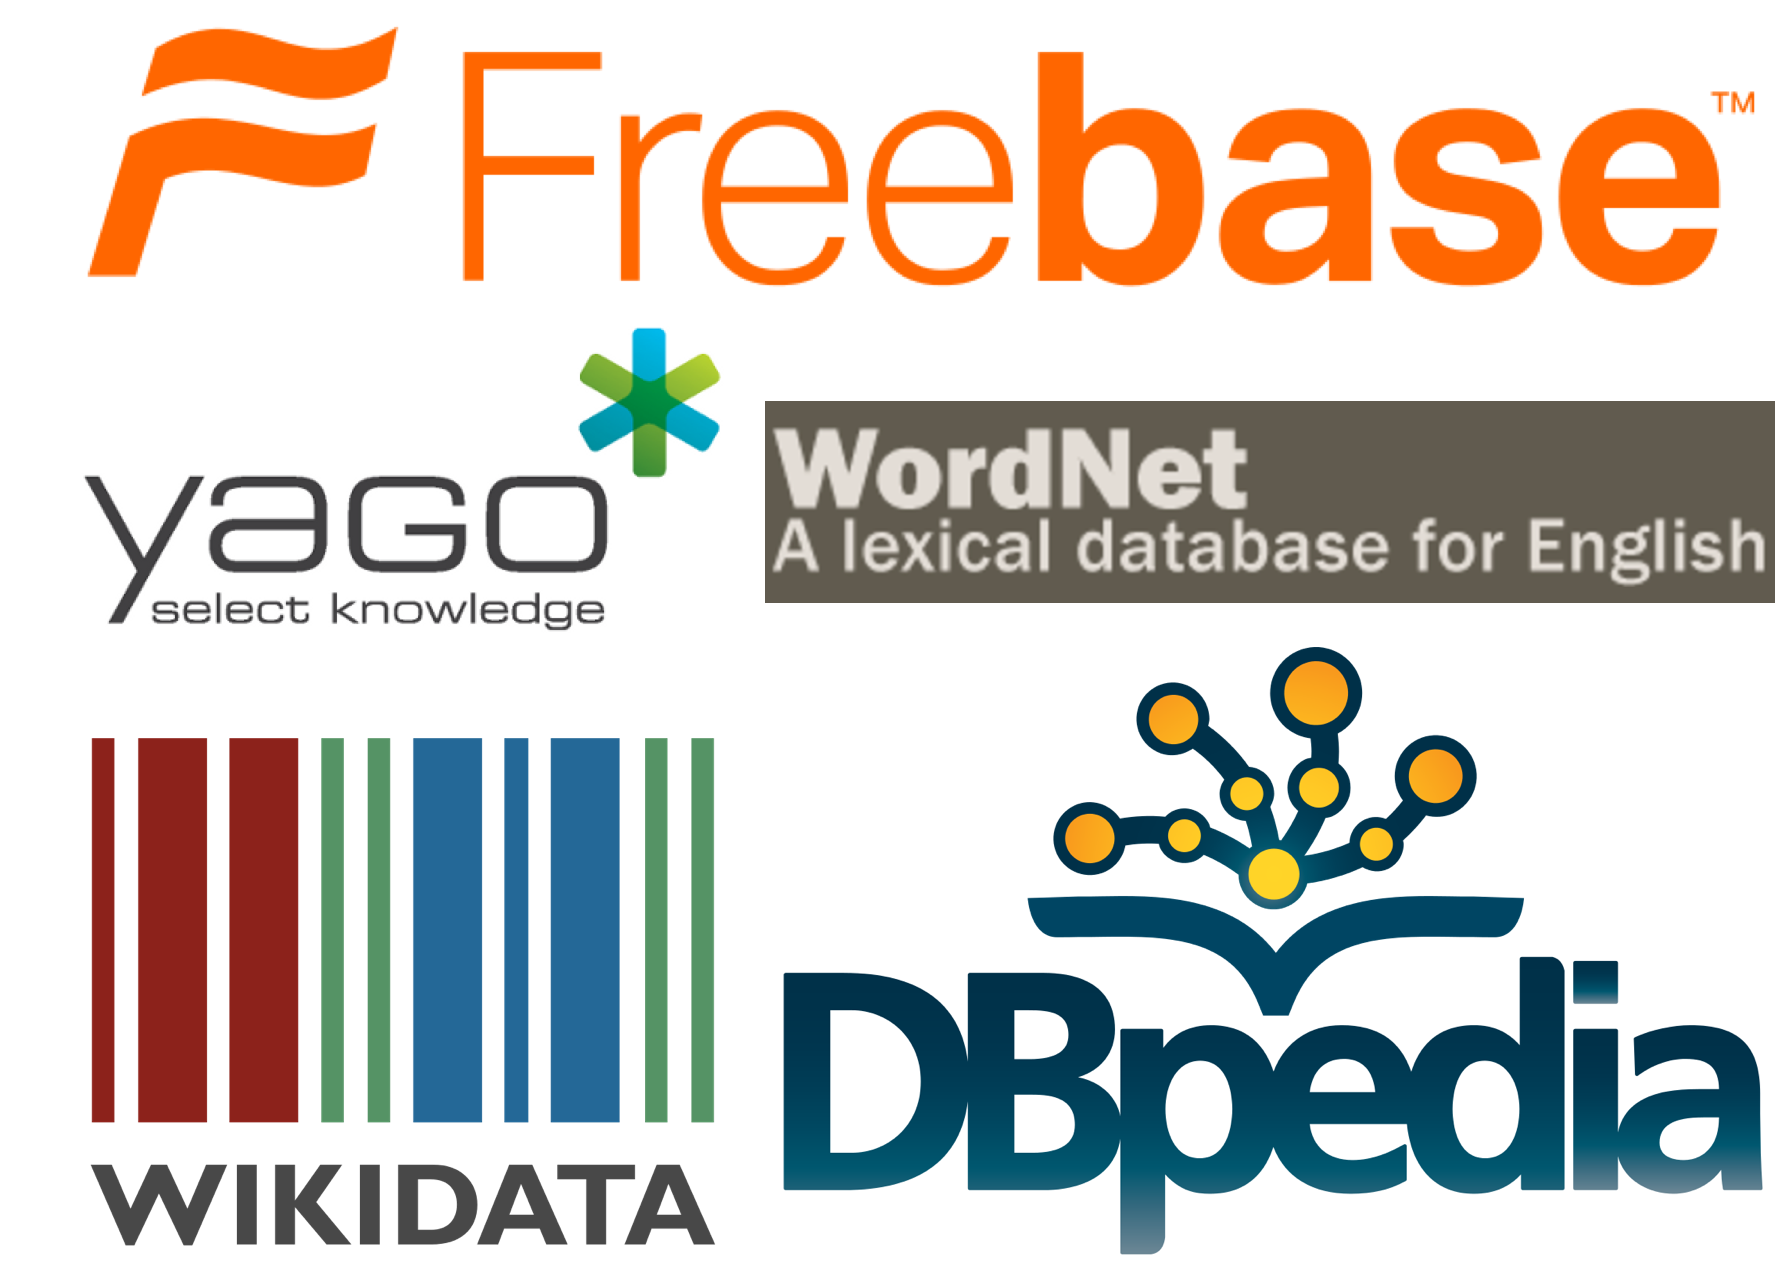
\includegraphics[width=0.8\columnwidth]{figures/ch1/KG_example.png}
\caption{一些常用的大规模知识图谱}
\label{ch1:KG_example}
\end{figure}

而随着时间的积累和相关工作者长期的工作,结合机器自动标注、专家标注和开放平台编辑校对等多种方法,现在已经构建出一些诸如图\ref{ch1:KG_example}中的高质量的大规模知识图谱,诸如 WordNet \cite{miller1995wordnet},YAGO \cite{hoffart2013yago2},DBPedia \cite{auer2007dbpedia},Freebase \cite{bollacker2008freebase},Wikidata \cite{vrandevcic2014wikidata} 以及 Knowledge Vault \cite{dong2014knowledge},并且被投入到部分相关研究场景中。截止到Freebase停止更新为止,Freebase中收集了超过 $2$ 亿个的实体,在其停止维护后这些信息正在被陆续迁移到 Knowledge Vault 和 Wikidata 中。经过维基社区的过滤和校对,截止目前,Wikidata中也有超过 $2600$ 万个高质量实体存在。与此同时,国内从事互联网领域尤其是和信息检索直接相关的企业也对知识图谱进行了投入,百度知心和搜狗知立方作为典型的中文知识图谱被构建出来并被使用到智能应用产品中进行知识驱动。

知识图谱将具象事物与抽象概念表示为实体,将实体之间的联系表示为关系,并以( \emph{头实体}, \emph{关系}, \emph{尾实体} )的形式表述知识。例如,“马克·吐温出生于佛罗里达州”在知识图谱中被表述为( \emph{马克·吐温}, \emph{出生于}, \emph{佛罗里达州} );“北京市下辖海淀区”在知识图谱中被表述为( \emph{北京市}, \emph{区划管辖}, \emph{海淀区} )等等。其中\emph{马克·吐温}、\emph{佛罗里达州}、\emph{北京市}、\emph{海淀区}即为实体,而\emph{出生于}、\emph{区划管辖}则是实体间的关系。一般来说,现在公开的知识图谱都是以这样的事实三元组(triple fact)的 形式抽象知识,并采用类似于万维网联盟(W3C)发布采用的资源描述框架(Resource Description Framework, RDF)进行储存。图\ref{ch1:google_kg_example}中展现的就是使用谷歌搜索``北京''时弹出的相关知识图谱。

\vspace{25pt}
\begin{figure}[h]
\setlength{\abovecaptionskip}{30pt} 
% \setlength{\textfloatsep}{60pt} 
\centering
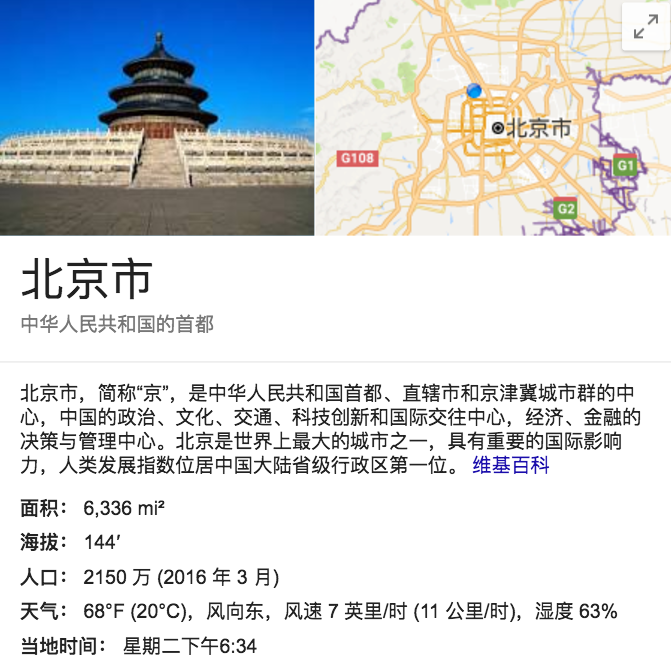
\includegraphics[width=0.6\columnwidth]{figures/ch1/knowledge.png}
\caption{日常搜索中出现的知识图谱}
\label{ch1:google_kg_example}
\end{figure}

伴随着上个世纪末互联网的蓬勃发展以及本世纪初信息技术的大量普及,在大量知识被整理进入知识图谱的同时,每天也有大量的知识产生。虽然当前的知识图谱离完善还差的很远,但以结构化形式存在于知识图谱中的知识也是相当惊人的多。而伴随着信息爆炸式增长以及日新月异的变化,海量的数据如何整理、存储、更新以及应用都是巨大的挑战。而这些知识图谱带来的技术诉求,其中很重要的一点就是如何以一个高效的方式进行知识图谱的表示。基于事实三元组集合的形式来表示知识图谱可以解决底层数据存储形式的问题,这与关系数据库的模式是十分相似的。但这样简单的抽象形式对于理解图谱、应用图谱乃至于依靠知识进行逻辑推理确是远远不够的。想要以高效的形式对知识图谱进行更高层的抽象,并且能够做到利用知识,这其中面临着许多难题:其一,是在计算效率上的问题。知识图谱往往以有向图的形式存在,以点为实体边为关系,这样的形式简单明了,却也需要图相关的算法来进行处理。早期基于图结构的图谱表示算法,其计算复杂度通常都非常高,以至于在大规模的知识图谱上难以适用。其二,知识图谱中实体和关系都很多,却没有实体数平方级别的事实三元组,这意味着知识图谱是稀疏图而非稠密图。与此同时,实体之间也相差很大,满足幂律分布。少部分高频实体和关系涵盖了多数的事实三元组,其余均是长尾部分。数据的稀疏性以及长尾分布也为模型设计带来巨大难度。

\vspace{25pt}
\begin{figure}[h]
\setlength{\abovecaptionskip}{30pt} 
\centering
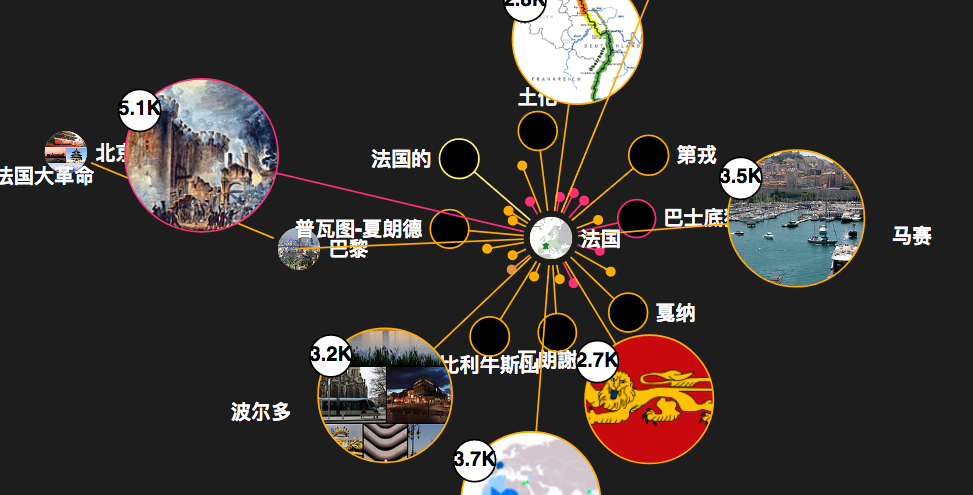
\includegraphics[width=0.9\columnwidth]{figures/ch1/space.png}
\caption{BabelNet 中与实体``法国''空间距离最近的实体}
\label{ch1:space}
\end{figure}

研究和解决抽象知识图谱过程中的计算复杂度与数据稀疏性问题,并将知识图谱表达为计算机可使用的模式,就是知识表示学习(Knowledge Representation Learning, KRL)的主要任务。近些年来,受到文本词向量的启发,将图谱进行分布式表示逐渐成为趋势。对于知识图谱来说,所谓的分布式表示(Distributed Representation),其实质就是将图谱中的实体和关系映射到低维度的连续空间中去。在映射空间上,对象之间的距离关系可以直接反映语义关联,比如语义相似的实体,其空间距离一般都十分相近。图\ref{ch1:space}展现的就是空间上与``法国''最相关的实体,数据来源于 BabelNet \footnote{http://babelnet.org/}。因为这个过程实际是将实体与关系的语义信息嵌入到低维度空间上,所以我们通常也将这个过程称为嵌入,得到的向量称为嵌入表示或直接称为嵌入(Embedding)。分布式表示一定程度上解决了之前提到的问题:首先,将知识图谱嵌入到低维度空间上,低维度的空间让实体与关系之间的语义关联计算更加便利,计算量也显著减少。其次,赋予每个实体与关系实数向量的表示,并且向量之间的空间关系来表示语义关联,很大程度上让知识图谱的分布不再稀疏。最后,以数值形式存在的知识图谱对于计算机来说比字符更容易理解和计算,将其作为其他各个应用模型的输入也变的容易起来。得益于知识表示学习在分布式表示上的有效推进,相关领域的工作也不断推陈出新,涌现了一批知识驱动为内核的模型。

虽然在知识表示学习的研究中已经有大量优秀的模型出现,且在实验数据集合上体现出了良好的性能。但是在实验环境中,数据集往往与实际的知识图谱相差甚远,通常只是公开大规模知识图谱的子集。通过实际对比可以发现,大规模的知识图谱无论在规模还是在分布上都比实验数据集合难处理的多,呈现出规模巨大、长尾突出的状态。与此同时,实验过程中模型的设计在突出性能考虑的时候往往忽略了模型复杂度,其工程实现也难以承受巨大规模的数据量。另一方面,知识图谱常常会与多源信息进行融合,尤其是与自由文本进行融合。以往的知识图谱与文本的融合模型均以串行形式进行融合,这也是很难在极大数据量的背景下进行训练与处理的。本文工作的主要目的就是立足于现有模型的基础上提出一套针对大规模知识图谱的表示学习框架、特征融合框架,在真实的大规模知识图谱上进行训练并得到优质的嵌入表示。

\section{相关资源}


 % \footnote{WordNet: http://wordnet.princeton.edu/ \\ YAGO: http://www.mpi-inf.mpg.de/departments/databases-and-information-systems/research/yago-naga/yago/ \\ DBPedia: http://wiki.dbpedia.org/ \\ Freebase: https://developers.google.com/freebase/ \\ Wikidata: https://www.wikidata.org/wiki/Wikidata:Main\_Page/} 


\section{研究内容}

\section{本文贡献}

  本文贡献总结如下:

  (1)通过底层实现的优化以及对知识图谱的划分,将以往的图谱模型改造成基于多线程的训练模型,在未来可以进一步衍生为分布式的训练模型,从而能够高效的对大规模知识图谱进行学习。
  
  (2)提出了加权点采样算法和位移负样例采样算法来取代原有的边采样及负例采样算法。能够在大规模图谱的幂率分布下对图中不同的实体和事实赋予不同的注意度,缓解幂率分布带来的长尾影响。二点采样的训练方式,可以在训练过程中尽可能的合并算术运算从而进一步加速。
  
  (3)采用了平行结合的方式与文本神经网络模型融合,对比于传统的串行结合方式,这样的模型能够更快的引入文本信息来丰富图谱内容并进行信息融合。在此基础上我们提出了一套联合学习的方法,使得图谱和文本的信息融合是双向的,图谱和文本模型融合之后两者都有显著效果提升
  
  (4)本文的相关工作提供了开源代码并对之前领域内的相关工作进行整理和总结,为之后相关领域需要使用知识图谱的后续研究打好基础,提供便利。

\section{论文组织}

  本文在第二章中综述知识图谱的发展轨迹,并对已有的知识图谱表示学习模型进行介绍、分析,从而能够对这一任务的相关工作进行梳理和总结。第三章介绍过去几年中被提出的知识图谱和文本模型的结合方法及相关任务,其中重点综述神经网络引入后深度模型的发展和联合学习模型的发展。第四章介绍我们提出的在大规模知识图谱背景下进行表示学习的框架,以及在此框架下和文本部分进行并行融合的联合学习方法。第五章介绍实验所用的数据并给出量化的评测结果,验证本文提出框架的准确性、可靠性和运行效率。

\chapter{基于并行的大规模知识图谱表示学习框架}
\label{cha:framework}

\section{简介}

% 正如我们之前提到

% % Knowledge graphs (KGs) are playing an important role in many applications such as question answering and web search. These applications require embeddings of entities and relations in KGs for efficient compution. A variety of effective methods have been proposed to embed KGs into continuous low-dimensional spaces. The implementations of these methods have been verified on small KGs, but not fast enough to embed large-scale KGs. To alleviate this issue, we present OpenKE, an efficient implementation framework for knowledge graph embedding via multi- threading training and some algorithmic design optimizations for acceleration. The evaluation results show that our frame- work can significantly improve embedding efficiency with comparable performance. We also provide embeddings of the exist- ing large-scale KGs, including Freebase and Wikidata, learned by our framework, which can be directly used for relevant ap- plications. Our toolkits and embeddings are released on our website 1.


% People construct various large-scale knowledge graphs (KGs) to organize structural knowledge about the world, such as WordNet \cite{miller1995wordnet}, Freebase \cite{bollacker2008freebase} and Wikidata \cite{vrandevcic2014wikidata}. These typical KGs are often organized in the format of multiple relational directed graphs. Nodes in KGs are corresponding to entities, and edges in KGs are corresponding to relations between these entities. Hence, the facts in KGs are usually recorded as a set of relational triples ($h$, $r$, $t$) with $h$ and $t$ indicating \emph{head} and \emph{tail} entities and $r$ indicating the relation between $h$ and $t$, e.g., (\emph{Mark Twain}, \texttt{PlaceOfBirth}, \emph{Florida}). After a long time of constructing and collating, information in the existing KGs is structural and clear, which can be used to help various applications get better performance, such as question answering and web search.

% \begin{figure*}[t]
% \centering
% \includegraphics[width=0.9\linewidth]{3.jpg}
% \caption{The overall framework of OpenKE}
% \label{fig:joinglearning}
% \end{figure*}

% To incorporate KGs into these applications, we need to embed entities and relations as input. Meanwhile, though most existing KGs are large, they are far from completion, which is also partially solved by embedding KGs recently. Thus, a variety of representative approaches have been proposed to encode entities and relations into a continuous low-dimensional space based on the network structure of KGs, such as graph-based models \cite{lao2010relational,lao2011random}, tensor-based models \cite{socher2013reasoning, nickel2016holographic} and translating models \cite{bordes2013translating,ji2015knowledge,ji2016knowledge}. TransE \cite{bordes2013translating} is a typical translating models, which regards the relation $r$ in each fact ($h$, $r$, $t$) as a translation from $h$ to $t$ within the low-dimensional space, i.e., $\textbf{h} + \textbf{r} = \textbf{t}$. Because TransE is an effective and efficient method that possesses good performance, it has many extensions, including TransH \cite{wang2014transh}, TransR \cite{lin2015learning}, TransD \cite{ji2015knowledge}, etc. 

% Although these translating models have achieved great results on small benchmark datasets, the existing implementations of these models are often single-thread and very time-consuming for training, which can not work well for embedding large-scale KGs. To learn large-scale knowledge graph embeddings, we propose some optimization methods. The optimization methods of our works are threefold. First, we design a unified framework to accelerate TransE and its extensions. The framework separates the overall KG into several parts and adopts these models for multi-threading training. We also propose the offset-based negative sampling to replace origin negative sampling algorithms in this framework. The new sampling mechanism can merge arithmetic operations for acceleration. Second, for some specific models, we also implement them by TensorFlow \cite{Abadi2016TensorFlow} based on our framework to build a convenient platform to run models on GPUs \footnote{https://github.com/thunlp/TensorFlow-TransX}. Third, besides the toolkits, we also provide pre-trained embeddings of large-scale KGs by this framework. The embeddings can be used directly for other works.

% We name our works as OpenKE. The experiment results show that OpenKE achieves great speedup ratio without harming the accuracy and efficient enough to learn large-scale KGs.





% \section{相关工作}

% 知识表示学习的代表模型主要包括距离模型、
% 双线性模型、神经张量模型、矩阵分解模型、翻译 模型等。

  
%     \subsection{早期的表示模型}
  
%     \subsection{基于张量的表示模型}
%       \subsubsection{RESACL}
%       \subsubsection{NTN}
%       \subsubsection{Hole}
%     \subsection{基于平移的表示模型}
%       \subsubsection{TransE}
%       \subsubsection{TransH}
%       \subsubsection{TransR}
%       \subsubsection{TransD}



\section{算法框架}

在这一章节内容里,我们主要介绍我们设计出的开放式知识图谱嵌入结构 OpenKE。内容包括 OpenKE 在并行模式下实现的大规模知识图谱表示学习框架,以及已有的知识图谱模型在框架 OpenKE 下进行实现和融合的具体方式和实施细节。整体的模型骨架我们可以在图\ref{fig:openke}中看到。在整个框架中,底层操作和上层模型是独立的,上层模型可以自由选择和适配,而底层结构则是我们进行了大量优化之后的并行架构。进一步讲,这样一个解耦合的框架使得一个新提出的模型也可以在无需过多关注底层的情况下得到高效实现,具有高自由度和高效率的特点,这些都将在之后的内容里详细铺开。当然,在介绍具体细节之前,我们先引入一些符号体系和重要概念。


\begin{figure*}[h]
\centering
\includegraphics[width=1.0\linewidth]{figures/ch2/3.jpg}
\caption{基于并行的大规模知识图谱表示学习框架 OpenKE 的结构示意图}
\label{fig:openke}
\end{figure*}

\subsection{符号体系和重要概念}

我们将整个知识图谱定义为一个由实体集、关系集和事实三元组集合共同组成的大集合,即$G = \{E, R, T\}$,这里$E$、$R$和$T$分别表示实体集合、关系集合和事实三元组集合。对于事实三元组集合中的任意事实$(h, r, t) \in T$,这个三元组表明头实体$h \in E$和尾实体$t \in E$之间存在一个逻辑上的关联$r \in R$。由于表示学习会将实体和关系都嵌入到连续空间中去并用对应的向量来表示他们的语义信息,所以对于任意的实体或者关系$h, t \in E$或$r \in R$,我们都用它们的加粗字母$\mathbf{h}, \mathbf{t}, \mathbf{r}$来表示它们的向量,这里的向量也可以称为嵌入、嵌入向量、表示、嵌入表示等。

\subsection{知识图谱表示学习模型}

对于知识图谱表示学习,模型需要做的就是将实体和关系嵌入到连续空间中,从而利用空间向量来表达它们之间存在的语义关联。在这里,我们先以一个统一的数学视角来归纳这些模型方法,从而方便之后在底层上进行统一的实现。然后我们接着给出在具体实现时,以 TransE 为代表的平移模型各自之间的不同之处。

在知识图谱表示学习模型中,通常先定义一个能量函数来衡量事实三元组的合理程度。更准确的说,对于任意一个给定的三元组$(h, r, t)$,模型会为之定义一个能量函数$S(h, r, t)$。如果三元组是合理的,比如$(h, r, t)\in T$,此时的能量函数将返回一个较低的值。相反,如果三元组是不成立的,那么能量函数则会返回一个较高的值。这个函数通常情况下和$h, r, t$在空间上的距离具有相关性,换句话说,存在关联的实体与关系在空间上也是相近的。

对于包括 TransE 及其一系列的拓展模型在内的基于平移的知识图谱表示模型,会定义一个潜在的向量表示$r_{ht}$来具象化头实体和尾实体$(h, t)$之间的潜在关系。这些模型之所以叫做基于平移的表示模型,是因为它们都遵循``关系在空间中是实体向量间的平移变换''这个基本假设。在这个假设下,如果三元组成立,那么会有潜在向量$\textbf{r}_{ht}$和显式的关系向量$\textbf{r}$在空间上极为接近。换句话说,我们获取头实体和尾实体之间关系的过程,就是一个寻找与潜在关系向量$\textbf{r}_{ht}$在空间上最近的关系向量的过程,由此我们将能量函数定义为两者的空间距离:
\begin{align}
\label{eq:energy functions}
S(h, r, t) & = \lVert \textbf{r} -  \textbf{r}_{ht} \rVert_{L1/L2}
\end{align}
这里,能量函数$S(h, r, t)$可以用L1距离衡量,也可以用L2距离衡量。在能量函数的基础上,我们可以进一步得到一个基于边界值优化的损失函数来作为我们的训练目标,并有如下公式:
\begin{align}
\label{eq:loss}
& \mathcal{L}(G) = \sum_{(h,r,t) \in T} \sum_{(h',r,t')\in T'} \big[ \gamma + S(h,r,t) - S(h', r, t') \big]_{+}
\end{align}
这里,$[x]_{+}$是这样一个函数,如果$x$是正数的话,那么返回值就是$x$,反之返回值为$0$。$\gamma > 0$是一个边界值,用来约束损失函数的训练。$S(h, r, t)$是正例三元组的能量函数得分,而$S(h', r, t')$是负例三元组的能量函数得分,$T'$是负例三元组的集合。这样的损失函数表明,我们希望正确的三元组和负例三元组的能量函数尽可能拉开差距,但又不能使训练过拟合,所以选定一个边界值并在其范围内进行最大化区分度的训练,这也是这些模型一脉相承的设计思路。而对于负例三元组集合$T'$有:
\begin{equation}
T' = \{(h',r,t)\}  \cup \{(h,r,t')\},
\end{equation}
负例三元组集合是通过将正例三元组$(h, r, t) \in T$中的实体替换成其他实体集合中的实体$h', t' \in E$来构造的。

在有了上述统一的损失函数和训练方法之后,我们可以基于几乎相同的边界值训练模式在我们的框架中来实现 TransE \cite{bordes2013translating}、TransH \cite{wang2014transh}、TransR \cite{lin2015learning}、TransD \cite{ji2015knowledge} 等诸多模型。这些模型主要的区别在于它们潜在关系向量$\textbf{r}_{ht}$计算方式的不同,其余部分和上述模型归纳一致。对于这些模型之间的区别和变化,我们接下来将详细罗列并介绍。

\textbf{TransE.} 在 TransE 中,对于每个三元组$(h, r, t)$,我们定义出以下的潜在关系向量$\textbf{r}_{ht}$和能量函数$S(h,r,t)$:
\begin{align}
&\textbf{r}_{ht} = \textbf{t} - \textbf{h},  \\\nonumber
&S(h, r, t) = \lVert \textbf{h} + \textbf{r} - \textbf{t} \rVert_{L1/L2}
\end{align}
由此可以看出,所谓的平移假设,实际上就是希望空间上满足$\mathbf{h}_r + \mathbf{r} \approx \mathbf{t}_r$。

\textbf{TransH.} 在 TransH 中,对于每个给定的实体,其在不同的关系环境下具有不同的嵌入表示。对于每个三元组$(h, r, t)$,我们定义出以下的潜在关系向量$\textbf{r}_{ht}$和能量函数$S(h,r,t)$:
\begin{align}
&\textbf{h}_r = \textbf{h} - \textbf{w}_r^{\top} \textbf{h} \textbf{w}_r, \\\nonumber
&\textbf{t}_r = \textbf{t} - \textbf{w}_r^{\top} \textbf{t} \textbf{w}_r, \\\nonumber
&\textbf{r}_{ht} = \textbf{t}_r - \textbf{h}_r,  \\\nonumber
&S(h, r, t) = \lVert \textbf{h}_r + \textbf{r} - \textbf{t}_r \rVert_{L1/L2}
\end{align}
这里$\textbf{w}_r$是一个归一化之后的向量,用来作为关系$r$所在平面的法向量。

\textbf{TransR.} 在 TransR 中,实体和关系是在不同的空间中被学习得到的,并且实体之间的平移性质是在关系向量所在的空间中进行的。对于每个三元组$(h, r, t)$,我们定义出以下的潜在关系向量$\textbf{r}_{ht}$和能量函数$S(h,r,t)$:
\begin{align}
& \textbf{h}_r = \textbf{M}_r \textbf{h} , \\\nonumber 
& \textbf{t}_r = \textbf{M}_r \textbf{t} , \\\nonumber
& \textbf{r}_{ht} = \textbf{t}_r - \textbf{h}_r,  \\\nonumber
& S(h, r, t) = \lVert \textbf{h}_r + \textbf{r} - \textbf{t}_r \rVert_{L1/L2}
\end{align}
这里$\textbf{M}_r$是关系$r$的映射矩阵,用来将实体从实体空间映射到关系空间中,以方便平移性质的实现。

\textbf{TransD.} 在 TransD 中,实体和关系同样是在不同的空间中被学习得到的。TransD 和 TransR 是十分相似的,但是其采用了动态的映射矩阵来进行映射。对于每个三元组$(h, r, t)$,我们定义出以下的潜在关系向量$\textbf{r}_{ht}$和能量函数$S(h,r,t)$:
\begin{align}
&\textbf{h}_{r} = \textbf{M}_{rh}\textbf{h}, \\\nonumber
&\textbf{M}_{rh} = \textbf{r}_p\textbf{h}_p^{\top}+\textbf{I}, \\\nonumber
&\textbf{t}_{r} = \textbf{M}_{rt}\textbf{t},  \\\nonumber
&\textbf{M}_{th} = \textbf{r}_p\textbf{t}_p^{\top}+\textbf{I}, \\\nonumber
&\textbf{r}_{ht} = \textbf{t}_r - \textbf{h}_r,  \\\nonumber
& S(h, r, t) = \lVert \textbf{h}_r + \textbf{r} - \textbf{t}_r \rVert_{L1/L2}
\end{align}
这里$\textbf{r}_p$和$\textbf{h}_p, \textbf{t}_p$都是用来生成映射矩阵$\textbf{M}_{rh}$和$\textbf{M}_{rt}$的映射向量。通过这样的映射方式,矩阵运算变为了向量运算,在保持了一定映射性质的情况下加快了整体训练速度。


\begin{algorithm}[t]
  \caption{并行学习伪代码}
  \label{algo1}
  \begin{algorithmic}[1]
        \Require 

        实体和关系集合$E, R$,

        训练三元组$T = \{(h, r, t)\}$,

        边界值$\gamma$,嵌入空间维度,

        训练轮数$epoches$,线程数$threads$,一批次训练数据量$batches$。
        \State \textbf{初始化} 

        $\textbf{e} \leftarrow $ uniform$ ( -\frac{6}{\sqrt{k}}, \frac{6}{\sqrt{k}}) $,对于任意$e \in E$;

        $\textbf{r} \leftarrow $ uniform$ ( -\frac{6}{\sqrt{k}}, \frac{6}{\sqrt{k}}) $,对于任意$r \in R$。

    \State \textbf{初始化}

    其他参数,比如:

    TransH 的$\textbf{w}_r$;

    TransR 的$\textbf{M}_r$;

    TransD 的$\textbf{r}_p, \textbf{h}_p, \textbf{t}_p$。
    
    \For {$i \leftarrow $ $1$ to $epoches$}
      \State 在每一个线程中:
      \For {$j \leftarrow $ $1$ to $batches/threads$}
      \State 采样正例 $(h, r, t)$
      \State 采样负例 $(h', r, t')$
      \If{$\gamma + S(h, r, t) - S(h', r, t') \textgreater 0$}
      \State \textbf{更新梯度} $\nabla \big[ \gamma + S(h,r,t) - S(h', r, t') \big]_{+}$
      \EndIf
      \EndFor
      \EndFor
    \State \textbf{返回} 训练得到的实体嵌入和关系嵌入
  \end{algorithmic}
\end{algorithm}

\subsection{并行结构}

在统一了各个知识图谱表示学习模型的形式之后,我们可以发现,这些模型除了上层的能量函数计算方法略有差距外,整体的底层结构,包括采样算法在内都是一致的。所以我们的框架在这些已有模型的底层基础之上,修改了部分结构以便于进行算法加速。其中极为重要的一点就是将知识图谱上的数据划分为若干部分训练三元组集合,并将模型改造成多线程形式来处理每一部分的集合。这样一个并行的学习方法在算法\ref{algo1}中给出了伪代码。

我们的并行学习结构采用的是基于数据并行的多线程机制,并且以此为基础实现了两种梯度更新的策略来训练模型。其中一种方法是通过无锁策略实现的,即所有的线程共享同一块内存空间,优化损失函数时可以实时地将导数反馈到内存中。因为没有加锁,所以在这个策略下,多个线程是可能出现竞争修改同一块内存的。所有线程共享统一的嵌入空间,直接更新嵌入而不进行同步操作,虽然这降低了梯度下降的质量,但整体上的速度提升效果非常明显。另一方面,我们还实现了一个中心同步梯度的方法。对于每个线程,它会计算其自身部分数据的梯度。当所有的线程都计算完毕后,中心会将整体的梯度进行加和,汇总后得到整体的梯度,然后这个结果将会被统一地反馈到实体和关系的嵌入向量或者其他参数上。

值得注意的是,同样的实体对或者实体关系对,可能在同一训练周期内被不同的线程同时计算到,这些重复运算是可以避免的,所以我们也合并了这些算术运算以便进一步加速我们的底层框架。



\begin{algorithm}[t]
  \caption{基于位移的负例采样算法}
  \label{algo2}
  \begin{algorithmic}[1]
      \Ensure 将所有实体$e \in E$映射为连续整数编码$num_e \in \{0, ..., \lVert E \rVert  - 1\}$。
        \Require 

        需要替换的三元组$(h, r, t)$,

        所有和$h, r$匹配的尾实体集合$E_{hr} = \{t|(h,r,t)\in T\}$。

        对于任意实体$e \in E_{hr}$,我们用其整数编码来进行排序,其在$E_{hr}$中的排名为$rank_e \in \{0, ..., \lVert E_{hr} \rVert  - 1\}$。
        \State $p \leftarrow $ rand$(0, \lVert E \rVert - \lVert E_{hr} \rVert)$
        \State $\hat{e} = \mathop{\arg\max}_{e \in E_{hr}} (num_{e}-rank_{e})$,这里需满足 $num_{e}-rank_{e} \leq p$,$num_{e}-rank_{e}$具有偏序关系所以可用二分来解决。
        \State \textbf{返回} 生成的负例三元组$(h, r, t')$,这里$t'$有$num_{t'} = p + rank_{\hat{e}}$
  \end{algorithmic}
\end{algorithm}


\subsection{基于位移的负例采样算法}

对于 TransE 及其一系列的拓展模型,它们的优化过程都是以最小化其基于边界值的损失函数而进行的,即最小化式\ref{eq:loss}。从大量的实践中我们发现,负例三元组的选择对最后的模型效果有着至关重要的影响。在前文介绍的负例三元组生成模式下,负例三元组集合$T'$是通过随机使用$E$中实体替换正例三元组的头尾实体来构建的。由于很多关系并不是一对一的模式,这意味着这套替换机制有可能用另一个正确的实体替换了当前的实体,$T'$中极有可能含有一些$T$中出现过的三元组。举个例子,替换机制将(\emph{美国},\emph{总统},\emph{奥巴马})替换为(\emph{美国},\emph{总统},\emph{克林顿}),两者都是正确的三元组。在实际处理中,如果替换实体之后生成的三元组在$T$中出现,那么这个三元组将不会被用作负例来处理。因此,在原有的负例采样算法中我们会花费大量时间来检验采样出的三元组是否在$T$中出现。为了优化此处的时间复杂度,我们提出了基于位移的负例采样算法来直接生成负例而无需进行任何检验。我们以替换尾实体为例,将该算法伪代码罗列在算法\ref{algo2}中。

在算法操作过程中,对于所有实体,我们用从$0$开始的连续的整数定义它们的整数编码,并且以此排序来使得实体集合具有序列性质,之后我们的各项操作都可以建立在这些整数编码之上。在替换过程中,我们首先随机一个编码。接着,我们采取了这样一个采样思路——如果存在非候选项(即$E_{hr}$中不能用来替换的实体),其整数编码落在随机数的范围内,我们就在随机编码的基础上加对应数量的偏移,从而将所有的非候选项都错开,并得到一个负采样的三元组。直观上讲,这个方法就是将所有的实体排列在一条线上,其中不能替换的实体会将整个直线划分为若干个线段,如果随机落点落在某个线段内则可以直接返回,如果随机落点出现问题落在顶点上的话,我们就将落点偏移使得落点只会在线段之内,这样生成的三元组是一定不会在$T$中出现的。

\section{实验设计与结果分析}

我们选取了知识图谱上的链接预测任务来进行框架性能的评测。在这里,我们一方面会对我们的框架 OpenKE 进行各种性能上的测试,另一方面我们会将结果与一个已经被广泛使用的工具包 KB2E \footnote{https://github.com/thunlp/KB2E}进行对比来体现 OpenKE 的高效性。KB2E 是 Lin 等人\cite{lin2015learning} 在论文发表后开源的工具包,其中实现了 TransE、TransH以及其自身工作 TransR在内的诸多知识图谱表示学习模型。KB2E 因为效果稳定而在很多工作中被使用,并且开源在 Github 上可以直接被获取。

在实验部分,所有的测试都是在$16$GB内存的单机上进行的,处理器为 Intel Core i7-6700K,拥有$4$个核心、$8$个线程,处理器的基本频率为$4.00$GHZ。

\subsection{实验数据集}

在实验中,我们选取了 FB15K 和 WN18 \footnote{https://everest.hds.utc.fr/doku.php?id=en:transe}这两个数据集合来进行测试。数据集合 FB15K 和 WN18 是知识图谱表示学习模型的主要评测基准,并在过去的大量工作中被广泛使用。这两个数据集合都是从公开的大型知识图谱中经过采样得到的子集,其中 FB15K 的内容是从 Freebase 中抽取出的,WN18 的内容是从 WordNet 中抽取出的。我们在表\ref{tab:statistics-of-FB15K}中详细罗列了 FB15K 和 WN18 的整体数据细节。

\begin{table}[htb]
\centering
\caption{FB15K 和 WN18 的数据细节}
\scalebox{1.0}{
\begin{tabular}{|c|c|c|c|c|c|}
\hline
Dataset & Relation & Entity & Train & Valid & Test \\ \hline
FB15K   & 1,345           & 14,951            & 483,142 &50,000 &59,071 \\ \hline
WN18   & 18           & 40,943            & 141,442  &5,000 &5,000 \\ \hline
\end{tabular}}
\label{tab:statistics-of-FB15K}
\end{table}

\subsection{实验与模型参数设置}
为了与之前的模型以及对应论文中公布的实验结果能够合理地进行对比,我们在实验参数的设定上遵循了之前知识图谱表示学习模型通用的办法。经验上,我们选择了边界值$\gamma = 4$来训练 WN18 下的各个模型,而对于 FB15K 我们则用$\gamma = 1$作为训练的边界值。在之前一些工作的实验中,TransE、TransH 以及 TransR 在$50$维上表现明显,TransD 在$100$维度上表现明显,所以我们将 TransE、TransH 以及 TransR 的嵌入向量维度设置为$50$,而将 TransD 的嵌入向量维度设置为$100$。无论是 FB15K 还是 WN18 我们均训练所有的模型$1000$轮以控制拟合的程度相对一致,且一轮训练会将数据划分为$100$批来进行处理。


\subsection{实验评估方式}
在 TransE \cite{bordes2013translating} 被提出时,链接预测就作为重要的评测方式来度量模型的嵌入表达能力。其评测方式为:给定一个头实体和关系的组合$(h, r, ?)$来预测对应的尾实体,或者给定一个尾实体和关系的组合$(?, r ,t)$来预测对应的头实体,预测的依据则是模型根据知识图谱结构学到的嵌入表示。在具体实施细节上,对于任意给定的测试三元组$(h, r, t)$,我们枚举所有的实体来替换头实体$h$以及尾实体$t$,并使用式\ref{eq:energy functions}计算能量得分,之后按照升序排列。根据我们归纳出的模型数学性质,$(h, r, t)$如果成立的话,其得分应当比替换后的三元组得分要低,即$h, t$的隐关系向量$\textbf{r}_{ht}$和$r$的向量在空间上是最接近的。这里我们仍然举个例子来说明,如补全三元组(\emph{?},\emph{著作},\emph{威尼斯商人})时,意味着我们在回答``《威尼斯商人》是谁的著作?''这个问题,这时我们要把所有的实体都尝试一下并给出对应的得分,如果模型合理的话,\emph{莎士比亚}被带入时会得到最优的评分。

和之前提到的相关工作一样,我们使用正确实体能量得分排在前十的比例来衡量预测质量,我们将这个结果称为$10$预测命中率(Hits@10)。因为我们需要的是模型整体的预测效能,并且从实践中来看$1$命中很难做到,也不是很好对模型质量进行细粒度区分,所以过去的模型和我们都选择了$10$预测命中率来进行实验。此外,我们也报告了正确实体的平均排序名次(Mean Rank),这个指标结果一定程度上直观体现了整体向量的学习质量。

我们之前也提到过,一个通过替换实体得到的新三元组很有可能是图谱中存在的正例三元组,该三元组其实不应当被算作是错误而存在。如需补全三元组(\emph{美国}, \emph{总统}, \emph{?})时,意味着我们在回答``美国总统是谁?''。如果三元组本身是(\emph{美国},\emph{总统},\emph{奥巴马}),但将\emph{奥巴马}替换成\emph{华盛顿}后有一个更好的评分,这并不能看作是一个失败的预测,甚至是模型低能的体现,毕竟(\emph{美国},\emph{总统},\emph{华盛顿})也是成立的。所以在替换完实体之后,在排名之前,我们将这些正确的三元组过滤掉,然后进行之前的 Hits@10 和 Mean Rank 的指标评估,这个结果我们称之为``Filter'',而没有经过过滤操作的结果我们称之为``Raw''。

在训练过程中,当替换三元组的实体时,我们遵循 Wang \cite{wang2014transh} 提出的两种方法,即 ``unif'' 和 ``bern''。``bern'' 采用不同概率来替换头尾实体,对于非一对一的关系,我们会对实体可能性较多的部分给予更多的关注和更大的概率来生成负例。而过去一贯等概率替换头或者尾实体的方法被命名为``unif''。使用不同的决策会导致不同的实验结果,对于所有的模型我们同时使用 ``unif'' 和 ``bern'' 两种决策来训练模型,并且在各项指标里选择较优的结果来代表模型的泛化能力。

\subsection{实验结果与分析}

对于涉及到的模型的实验结果,我们直接引用了对应论文里汇报的数据,并且记录为其对应模型名。在我们的框架 OpenKE 下实现的各个模型,其实验结果被命名为模型名加``OpenKE''后缀,比如 TransE(OpenKE)。由于我们会与工具包 KB2E 中实现的模型来进行效率对比,所以我们引入了 KB2E 中的 TransE,命名为 TransE(KB2E)。

所有的实验结果都罗列在表\ref{tab:performance_comparison1}之中。除此以外,我们还报告了在不同的线程设定之下,损失函数的下降曲线,不同模型在不同线程设置下的加速比,这些分别体现在图\ref{fig:loss}和图\ref{fig:speedup}中。



\begin{table*}[h]  
  % footnotesize
  \centering  
  \caption{链接预测的结果}  
  % \fontsize{7}{9}\selectfont  
  \label{tab:performance_comparison1}  
  \scalebox{0.94}{
    \begin{tabular}{|c|c c|c c|c|c c|c c|c|}  
    \hline    
    Data Sets&\multicolumn{5}{c|}{WN18}&\multicolumn{5}{c|}{FB15K}\\\cline{1-11}
    \multirow{2}{*}{Metric}&
    \multicolumn{2}{c|}{Mean Rank}&
    \multicolumn{2}{c|}{Hits@10(\%)}&
    \multirow{2}{*}{time(s)}&
    \multicolumn{2}{c|}{Mean Rank}&
    \multicolumn{2}{c|}{Hits@10(\%)}&
    \multirow{2}{*}{time(s)}
    \cr
    {}&Raw&Filter&Raw&Filter&{}&Raw&Filter&Raw&Filter&{}\cr
    \hline
  
    TransE(KB2E)&251&239&78.9&89.8&1674&210&82&41.9&61.3&3587\cr
    TransE(OpenKE)&273&261&71.5&83.3&12&205&69&43.8&63.5&42\cr
    TransE&263&251&75.4&89.2&-&243&125&34.9&47.1&-\cr\hline      
    TransH(OpenKE)&285&272&79.8&92.5&121&202&67&43.7&63.0&178\cr  
    TransH&318&303&75.4&86.7&-&221&84&42.5&58.5&-\cr\hline         
    TransR(OpenKE)&284&271&81.0&94.6&296&196&73&48.8&69.8&1572\cr
    TransR&232&219&78.3&91.7&-&198&77&48.2&68.7&-\cr\hline      
    TransD(OpenKE)&309&297&78.5&91.9&201&236&95&49.9&75.2&231\cr 
    TransD&224&212&79.6&92.2&-&194&91&53.4&77.3&-\cr\hline   

    \end{tabular}}  
\end{table*}

\begin{figure*}[h]
\small
\begin{minipage}[]{0.5\linewidth}
\centering
\setcaptionwidth{2.8in}
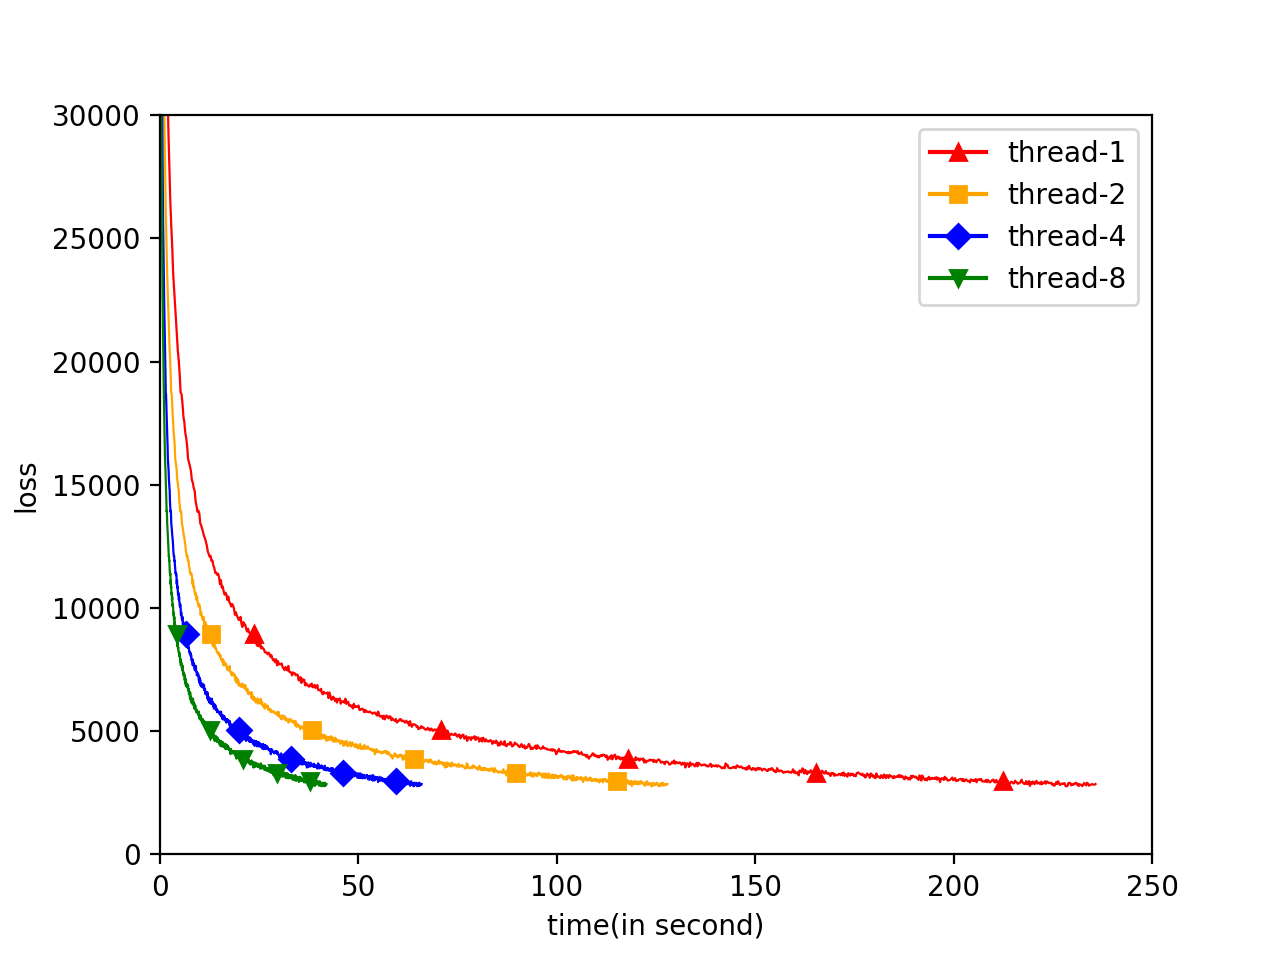
\includegraphics[width=1\linewidth]{figures/ch2/FB15-transE-loss.png}
\caption{在不同线程设定下,TransE 在 FB15K 上的损失函数走向}
\label{fig:loss}
\end{minipage}
\begin{minipage}[]{0.5\linewidth}
\centering
\setcaptionwidth{2.8in}
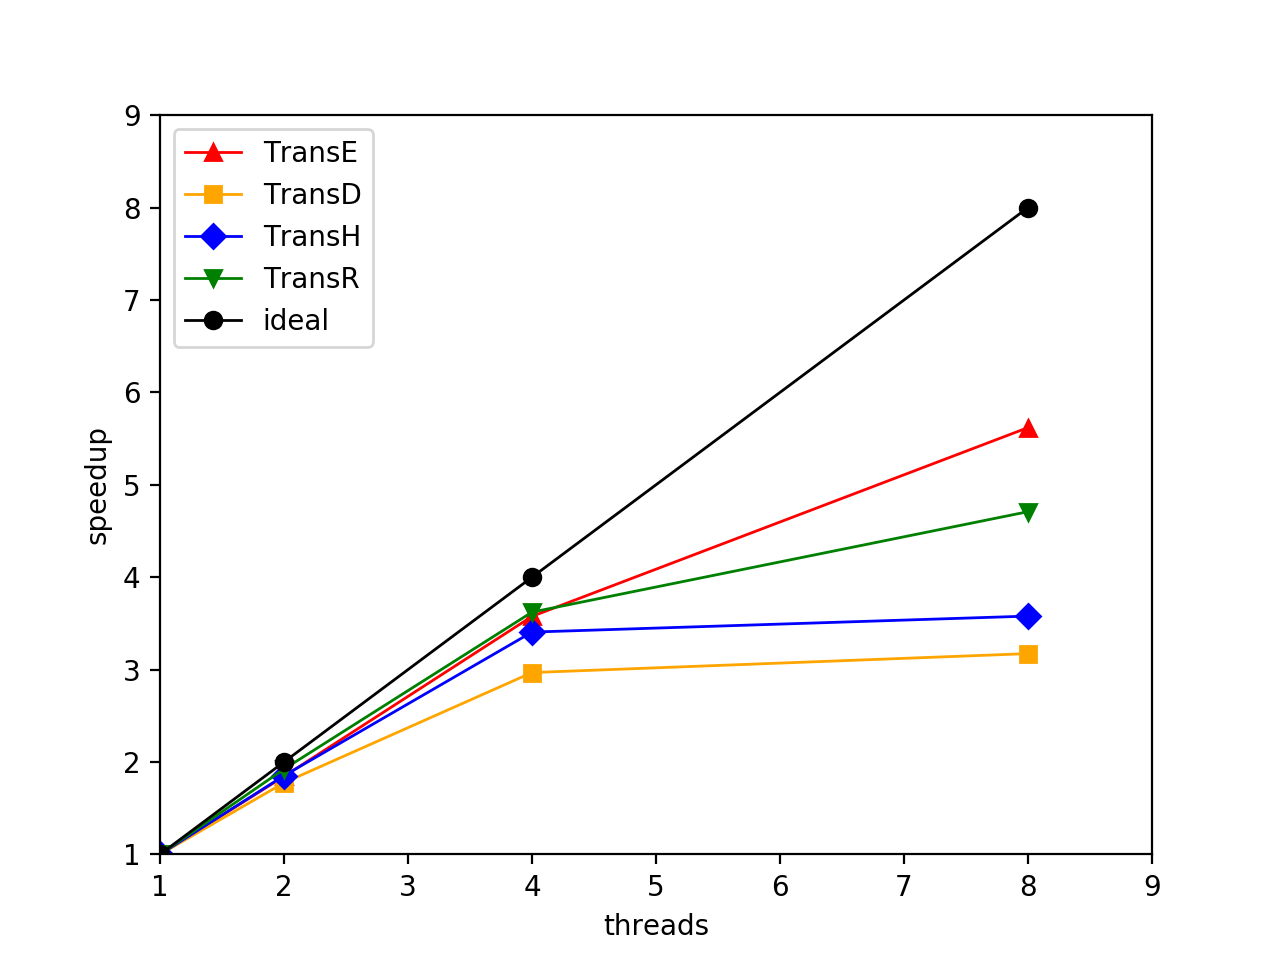
\includegraphics[width=1\linewidth]{figures/ch2/FB15K-transR-speedup.png}
\caption{在不同线程设定下,OpenKE 下不同模型的加速比曲线}
\label{fig:speedup}
\end{minipage}
\end{figure*} 

从这些结果我们可以发现:

(1) KB2E \cite{lin2015learning} 是一个对之前知识图谱表示学习模型非常有效的实现,其评测结果比论文原始结果要高出许多。而和 KB2E 相比,OpenKE 下学到的模型在时间上要短的多,并且效果也非常接近,这意味着 OpenKE 极大的优化了训练速率并且没有影响模型性能。从整体来看,TransE 在 OpenKE 上的实现比其在 KB2E 上的实现加速了85倍。这么大的加速比一方面是因为 KB2E 是一个底层单线程的框架,而我们的 OpenKE 却是基于数据并行的并行框架。但是在$8$线程的处理器上,即使是理想情况,即不计通信同步时间,多线程加速比的极限也不会高于$8$。所以,我们$85$倍的加速除了有多线程的贡献外,另一个重要的因素就是我们基于位移的负例采样算法和底层算术运算合并带来的积极作用。实际上,这些非算法结构上的优化对实际耗时的减少至关重要。


(2) 通过链接预测的结果,可以发现在我们的框架 OpenKE 下训练的模型,基本取得了与原始报告数据非常接近的准确度,并且在其中部分模型上,在 OpenKE 下实现可以获得略高的精度,这些现象和我们的预期是相符合的。因为我们的数据并行机制对在 OpenKE 下实现的模型没有影响,尤其是不会改变这些模型的数学性质,直观上讲我们的框架将一批数据分给若干个线程处理,而每个线程的处理方式和单线程是一致的。与其他模型相比,TransR 需要更多的时间来学习知识图谱的嵌入表示,这主要是 TransR 需要将实体通过映射矩阵投影到关系空间中,而矩阵运算其实是一个计算瓶颈,并且在CPU上很难解决。为了减轻矩阵运算带来的计算瓶颈,我们还在相同底层结构的框架上给出了 GPU 版本的模型实现。因为其模型性质和 CPU 版本是一致的,所以我们只是给出 GPU 版本的链接而不在实验中进行度量,链接附在本章节引言部分处。

(3) 伴随线程数的不断增多,损失函数下降需要的时间以及各模型和单线程相比的加速比都有了变化。从损失函数的下降曲线以及实际加速比曲线可以看到,多线程框架带来的优化以及耗时的下降非常的显著。当线程数小于$4$时,加速比与线程数几乎成正比,也基本接近理想的加速情况。当使用超过$4$个线程时,由于线程调度中的通信和同步,并行能力受到很大影响,加速比的上升速度开始逐渐缓慢甚至保持不变。这其中的影响因素主要来自于我们所采用的处理器。我们的处理器虽然有$8$个线程,却只有$4$个计算核心,这意味着在使用超过$4$个线程时,每个核心将需要负载至少两个的工作线程,线程的切片和通信过频会导致效率下降,所以出现了两个图表后半段加速比停滞的情况。实际上,如果采用更适合并发的处理器,这个停滞的现象将会在更多的线程被启用时才出现,而不是仅仅超过$4$个线程就接近瓶颈,这也启发我们在当前工作的基础上继续采用分布式而非单卡的框架来进行加速。

总的来说,各项评估结果表明,我们的框架成功解决了之前模型实现存在的巨大耗时问题,从而使得这些已经被提出的算法能够真正地对大规模的知识图谱进行表示学习。我们整合了这些模型底层的共通之处,使得新算法可以在不考虑底层繁琐细节的情况下也能得到高效实现。事实上,基于我们 OpenKE 的 TransE 只需耗时$18$个小时就可以训练整个 Wikidata 达$10000$轮左右,并可以获得一个稳定的嵌入表示。我们在引言部分介绍过,wikidata 是一个拥有超过$2500$万实体的巨大知识图谱。这些预先学习好的嵌入表示我们将其公开在网络 \footnote{http://openke.thunlp.org/} 上供直接使用。

\section{本章小结}

对于真正的大规模知识图谱表示学习问题,我们提出了一个有效的训练框架 OpenKE 以便在现有模型基础上进行改进,从而能够解决我们的需求。与此同时,我们也基于该框架提供了已训练完成的大规模知识图谱嵌入向量,使得部分应用可以直接使用而无需再去耗时训练向量。我们的框架采用了基于数据并行机制的并行学习方式,从而能够取得数倍的速度提升。除此以外,我们还提出了基于位移的负例采样算法以及部分基础算术运算合并来进一步加速训练。在实验部分,链接预测上的实验结果表明,在通用的评测数据上我们的底层设计可以帮助现有模型有效地提高效率。而各个模型也在不剧烈影响精度的情况下显著缩短了训练的时间。目前在我们 OpenKE 架构下,部分模型得到了高效复现并且已经能够在真实的大规模知识图谱上进行训练。在未来,我们还将探索并尝试在 OpenKE 的框架下实现更多的知识图表示学习模型。此外,在现有基于多线程的并行学习模式之外,我们还将尝试构建分布式架构来进一步解决规模和时耗问题。在我们的工作中,我们也基于 TensorFlow 来为 OpenKE 实现了一个相对简单的GPU版本,在我们未来的工作中,使用高效的GPU底层框架也是一个十分有意义的方向。

\chapter{基于并行的知识图谱与文本模型联合学习框架}
\label{cha3:jointlearning}

\section{章节引言}

我们之前介绍过,典型的知识图谱是一个多关系有向图,其节点对应于现实世界中的抽象实体,边对应于抽象实体间的复杂关联。知识图谱中的事实通常以关系三元组的形式存在,如$(h, r, t)$,$h$和$t$表示\emph{头}实体和\emph{尾}实体,$r$表示$h$和$t$之间的\emph{关系}。例如(\emph{马克吐温},\emph{出生于},\emph{佛罗里达州})。

不过目前的知识图谱还远远达不到完善的程度,尽管它们规模已经很庞大了。通常有两类任务来获取知识信息并以此拓展知识图谱,知识图谱填充以及关系抽取。知识图谱填充旨在通过图谱内部的网络空间结构来挖掘信息并推测新的事实三元组,其中包括了基于图结构的模型\cite{lao2010relational,lao2011random},基于张量的模型\cite{socher2013reasoning, nickel2016holographic},以及基于平移的模型\cite{bordes2013translating,ji2015knowledge}。与图谱填充技术不太一样,关系抽取主要是从自由文本中提取特征并用来抓取新的关系事实。在这个方向上,也有大量行之有效的工作出现。Surdeanu \cite{surdeanu2012multi}就提出了一套基于多实例和远距离监督算法的模型,成为现在大多数方法的雏形。近年来,随着深度学习的发展,Zeng \cite{zeng2014relation}使用卷积神经网络来嵌入语句特征,也获得了不错的结果。

虽然依靠的信息来源是不同的,但这两个方向的目标是一致的,即进行知识获取。因此,将知识图谱和文本语料进行融合来进行知识信息的获取是一个非常直接的想法,并且已经在过去的一些工作中被简单探索。Weston \cite{weston2013connecting}直接将两方面模型的能量函数进行加,从而最终的预测是涉及图谱和文本两方面信息的结果。Wang \cite{wang2014knowledge}提出了一个简单框架将文本的词向量和实体向量进行对齐。Toutanova \cite{toutanova2015representing} 则是从纯文本中提取文本关系并与关系向量对齐。这些模型要么只考虑了文本与图谱的部分对应关系,如单纯的实体文本对应或者关系文本对应,要么特征融合后仅仅解决了知识获取中单方面的任务,这意味着这些模型还有很多可改动的空间。另外这些方法图谱和文本的结合模式大都是串行的,神经网络巨大的运算量将会带来长时间的训练,在大规模数据上适用也值得商榷。

为了解决这些问题,我们提出了一个通用的联合框架可以同时融入知识图谱填充以及关系抽取的模型,并其联合方式是基于平行的,相比于串行联合在效率上提升很大。如图\ref{fig3:joinglearning}所示,该框架同时对单词、实体、关系以及文本关系进行了对齐,从而能够综合考虑文本和知识图谱的信息并发挥各自优势。此外,我们使用了深层神经网络与基于知识图谱的注意力机制来构建文本模型,而不是使用传统的语言分析来编码句子的语义,这非常适用于大规模文本尤其是掺杂有噪音的远距离监督抓取得到的文本。基于知识的注意力机制使用知识图谱的信息来选择语料中的最核心的句子来强化训练,与此同时,文本的关系特征也通过注意力机制反馈给图谱模型。因为只有强有力的图谱特征才能进行这样的筛选。我们的框架也是非常灵活的,大多数现有的基于嵌入式的图谱填充算法以及关系抽取算法都可以很容易地集成到框架之中。

我们在真实环境下的数据上进行了实验,其中知识图谱是从Freebase中提取获得的,而文本则是来源于纽约时代周刊的语料库。我们同时在知识图谱填充和关系抽取两个方向上进行实验评估。而实验的结果也表明,我们的框架可以有效地进行联合学习和特征融合,并获得嵌入更多信息量的知识和文本表示,其效果显著优于单一依靠图谱或者文本的基础方法。

\section{相关工作}

在本章节中,我们罗列了与框架相关的工作,包括知识图谱表示学习、文本关系表示模型、基于联合学习的知识获取模型以及基于注意力机制的神经网络模型,相关内容如下。

\subsection{知识图谱表示学习模型} 

对于知识图谱表示学习,已经有一些成熟的模型被设计出来,将图谱中的实体与关系嵌入到低维连续空间中,从而能够以数学形式刻画知识图谱的结构。Bordes \cite{bordes2013translating} 提出了基于平移的知识图谱表示学习模型 TransE,其基本假设就是将每个事实$(h, r, t)$中的关系$r$视为低维空间内的$ h$至$t$向量的平移,例如,$\textbf{h} + \textbf{r} = \textbf{t}$。尽管 TransE 的模型非常简洁,却能取得非常优异的结果,无论是效率上还是结果上。因此,大量的扩展模型也在 TransE 的基础上被提了出来,包括 TransH \cite{wang2014transh}、TransR \cite{lin2015learning}、TransD \cite{ji2015knowledge}等。除了基于平移的模型之外,基于张量的模型,诸如 RESCAL \cite{nickel2011three}、NTN \cite{socher2013reasoning}、HOLE \cite{nickel2016holographic},也是非常有效的模型。某种程度上,基于张量的模型比基于平移的模型表达能力要强一些。但是基于张量的模型训练缓慢,参数数量以及资源占用也非常大。出于时效性价比的考虑,我们将基于平移的模型 TransE 和 TransD 作为代表模型在我们的框架中进行知识图谱表示学习。

\subsection{文本关系表示学习模型}

大量的工作和模型也被提出,力图从大规模文本语料中提取关系事实。Mintz \cite{mintz2009distant} 在其工作中提出了远距离监督(Distant Supervised)模型,利用知识图谱自动标注文本数据,再利用自动标注的文本数据用以构建关系表示模型并进行关系抓取。之后,Hoffmann \cite{hoffmann2011knowledge} 在远距离监督模型的基础上提出了跨句合并机制,利用句子间的相关特征来服务抓取模型。实体间的关系往往不是唯一的,而Surdeanu \cite{surdeanu2012multi} 提出了多关系抓取模型 MIML 来解决这个问题。在最近的几年里,深度神经网络被使用在各个领域中,包括文本关系表示,其中有基于卷积神经网络的工作 \cite{zeng2014relation,zeng2015distant}、基于循环神经网络的工作 \cite{zhang2015relation}、长效记忆网络模型\cite{xu2015classifying,miwa2016end}。对于给定的句子以及句子中的实体,神经网络会将句子的语义编码为语义向量,而语义向量则可以帮助模型获取文本关系。与传统的模型相比,神经网络模型能够准确地捕获文本关系而不用进行过于复杂的语言分析和特征处理。出于时间效率上的考虑,在本工作中,我们应用卷积神经网络来嵌入文本关系。


\subsection{基于联合学习的知识获取模型}

也有一些工作尝试将知识图谱和文本语料联合在一起进行特征融合以及知识信息的获取。Weston \cite{weston2013connecting}提出了一个简单的算法。Weston将 TransE 和 文本模型进行简单结合,用文本模型的评分与知识图谱模型的评分加权和进行预测。虽然方法十分简单,但是在关系抽取上取得了巨大的成功和惊人的表现。之后,Wang \cite{wang2014knowledge} 提出了一套联合学习的框架,将词向量与知识图谱的实体向量进行关联,同步训练并在训练过程中共享参数,从而将文本特征与图谱特征进行融合。Xie \cite{xie2016representation}和 Wu \cite{wu2016knowledge} 使用神经网络将与实体相关的文本内容嵌入到图谱空间中去,从而可以强化图谱中实体的表达能力。Toutanova \cite{toutanova2015representing}使用文本依赖关系解析从纯文本中提取文本关系来增强图谱中关系嵌入的表达能力。 
在本工作中,我们结合现有的知识获取模型,建立一个统一的联合学习框架,使单词、实体和关系都进行对应,并且有别于以往串行结合的联合方式,我们采用平行的结合方式来增加训练速度。


\subsection{基于注意力机制的神经网络模型} 

注意力机制最早被Bahdanau\cite{bahdanau2014neural}在其神经机器翻译模型中使用,用来从神经网络的隐层向量里选择最重要的成分来强化训练且规避噪音。在关系抽取上,Lin\cite{lin2016neural}立足于以往的模型,通过跨句级别的注意力机制来减少远距离监督算法带入的噪音成分。在本工作中,我们提出了一种基于知识图谱的注意力机制。与Lin\cite{lin2016neural}不同,我们基于知识的注意力机制不是采用全局的注意力特征,而是使用图谱信息构建局部的注意力特征,这会在复杂的文本环境下更加有效和鲁棒。

\section{算法框架}
在这一章节的内容里,论文主要介绍我们提出的基于并行的知识图谱与文本模型联合学习框架。内容包括以下几点:(1)联合框架下知识图谱与文本表示的统一形式;(2)知识图谱表示学习模型;(2)文本关系表示学习模型;(3)基于知识的跨句注意力机制;(4)初始化及实现细节,整体的框架结构也可以在图\ref{fig3:joinglearning}中看到。从框架结构图中可以发现,在整个框架中,我们进行了大量的嵌入表示融合工作。这些融合工作包含了知识图谱与文本表示在模型形式上的统一,词与实体、关系与文本关系在嵌入向量上的统一等等。得益于这些统一的归纳与抽象,我们可以通过使用统一空间学习嵌入表示的方式来进行联合学习。联合学习支持模型间的参数共享,从而使得原本分离的模型在合并后可以相互影响并一定程度的促进各自效果提升。在介绍具体细节之前,我们仍然先引入一些符号体系和重要概念。

\begin{figure}[h]
\centering
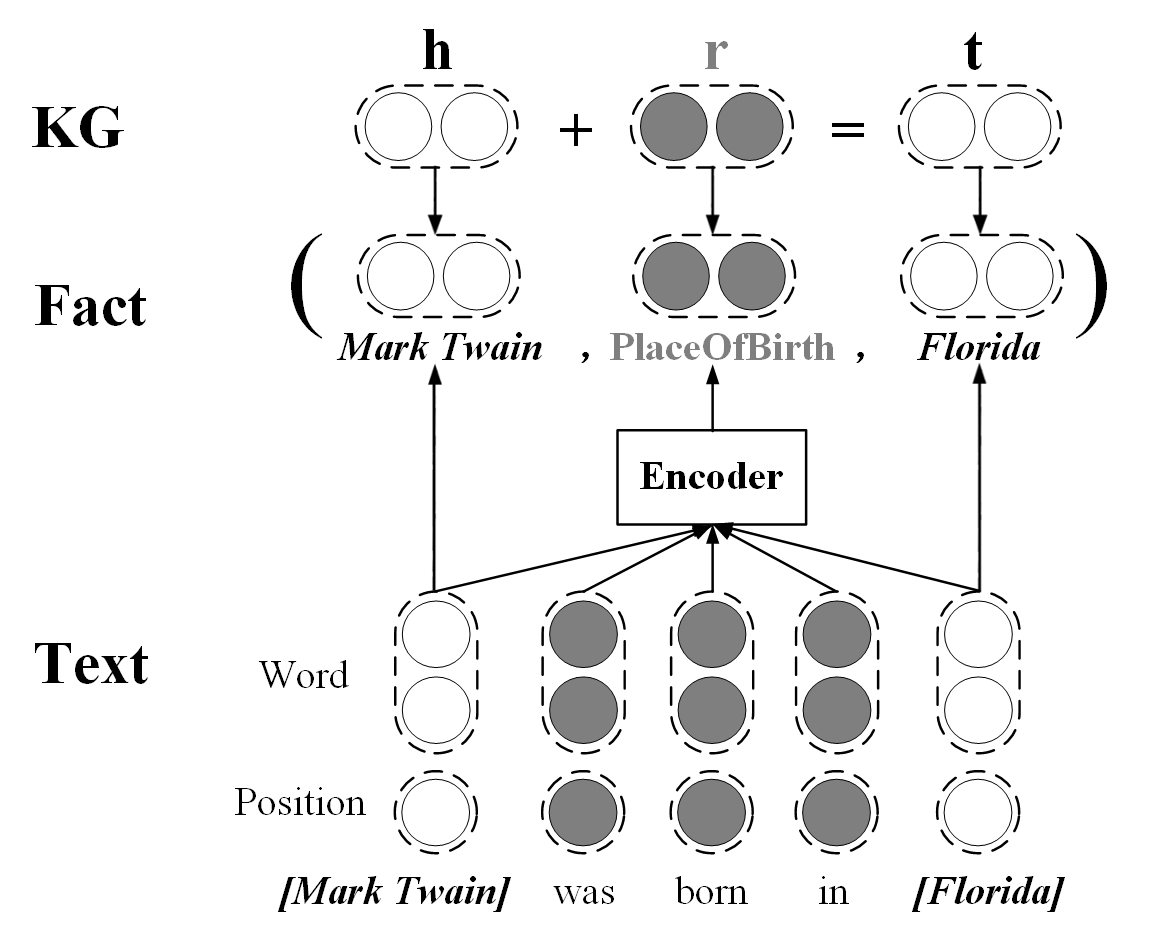
\includegraphics[width=0.9\columnwidth]{figures/ch3/joint.jpg}
\caption{基于并行的知识图谱与文本模型联合学习框架}
\label{fig3:joinglearning}
\end{figure}

\subsection{符号体系和重要概念}

与大规模知识图谱表示学习框架一样,我们在这里同样将整个知识图谱定义为一个由实体集、关系集和事实三元组集合共同组成的大集合,即$G = \{E, R, T\}$,这里$E$、$R$和$T$分别表示实体集合、关系集合和事实三元组集合。对于事实三元组集合中的任意事实$(h, r, t) \in T$,这个三元组表明头实体$h \in E$和尾实体$t \in E$之间存在一个逻辑上的关联$r \in R$。

同知识图谱$G$相对应的信息载体是文本语料。在这里,我们将文本语料定义为$D$。$D$是一个文本数据集合,集合中的基本构成元素为文本句子,而构成这些句子的单词集合被定义为$V$,即词汇表被定义为$V$。对于文本数据集合$D$中的任意一个句子$s$,$s$被定义为由若干词汇表$V$中单词构成的词语序列$s = \{w_1, \ldots, w_n\}, w_i \in V$,其中$n$为句子的长度也是词语序列中单词的个数。通过一些处理,在每个句子中,会有两个标注出的实体,并且句子本身的文本内容可以叙述标注实体间的潜在语义关联$r_s \in R$。对于文本实体和语义关系的具体标注方法将会在章节\ref{sec3:alignment}处被介绍。

由于表示学习模型会将实体和关系都嵌入到连续空间中,并用空间中对应的向量来表示他们的语义信息。所以,对于任意的实体或者关系$h, t \in E$或$r \in R$,我们都用它们的加粗字母$\mathbf{h}, \mathbf{t}, \mathbf{r} \in \mathbb{R}^{k_w}$来表示它们的向量,这里的向量也可以称为嵌入、嵌入向量、表示、嵌入表示等。对于词汇表中的任意单词$w \in V$,我们同样用加粗字母$\mathbf{w}\in \mathbb{R}^{k_w}$来表示其向量。$k_w$是这些单词、实体与关系嵌入表示的维度。

\subsection{联合学习的整体模式}
\label{sec3:joint}

对于整个联合学习框架来说,我们的设计目标就是让框架可以支持各个模型在统一的连续空间中同时训练,从而可以同步获得实体、关系及单词的嵌入表示。在训练过程中通过这样一个统一空间带来的联合约束,特征信息可以方便地在知识图谱和文本模型之间进行共享和传递。我们将所有的嵌入表示以及模型中涉及的参数都定义为模型参数,并用符号$\theta = \{\theta_E, \theta_R, \theta_V\}$来表示,其中$\theta_E, \theta_R, \theta_V$分别是实体、关系、单词的嵌入向量与相关参数。如果将我们对框架的性能要求形式化描述的话,模型需要做的就是找到一组最优的参数$\hat{\theta}$满足
\begin{equation}
\hat{\theta} = \mathop{\arg\max}_{\theta} P(G, D | {\theta}) 
\end{equation}
也即,
\begin{equation}
\hat{\theta} = \mathop{\arg\max}_{\theta} P(G, D | {\theta_E, \theta_R, \theta_V})
\end{equation}
这里$\theta_E, \theta_R, \theta_V$就是刚刚定义的嵌入与参数。$P(G, D | {\theta})$ 是一个定义出的条件概率,用来刻画在给定实体、关系与单词嵌入$\theta$的情况下,嵌入对图谱与文本的拟合能力、表达能力。更直观一点讲,模型的任务就是找到最好的嵌入表示能够最大程度的拟合给定的知识图谱结构以及文本语义信息。而条件概率$P(G, D | {\theta})$又可以进一步被分解为
\begin{equation}
\label{eq3:topeq}
P(G,D|{\theta}) = P(G|{\theta_E,\theta_R})P(D|{\theta_V})
\end{equation}

$P(G|\theta_E, \theta_R)$ 被用来从知识图谱$G$中学习结构特征,并得到实体和关系的嵌入表示。这个公式的物理意义就是希望模型能够最大限度的让知识图谱$G$中的事实概率变大,而图谱外的三元组概率变小,关于此部分的详细内容将会在章节\ref{sec3:kg}中展开。

$P(D|{\theta_V})$ 被用来从文本语料$D$中学习文本特征,并得到单词与语义关系的嵌入表示。这个公式的物理意义就是希望模型能够最大限度的让$D$中句子的语义信息与其描述的语义关系相对应,关于此部分的详细内容将会在章节\ref{sec3:relation}中展开。

根据物理意义,我们将知识图谱在参数下的条件概率$P(G|\theta_E, \theta_R)$定义为其包含事实的成立概率,将文本在参数下的条件概率$P(D|{\theta_V})$定义为语义信息与语义关系匹配的概率。我们对原概率式进行变换,得到
\begin{equation}
P(G|{\theta_E,\theta_R})  = \prod_{(h,r,t) \in G}P((h, r, t)|{\theta_E, \theta_R})
\end{equation}
以及
\begin{equation}
P(D|{\theta_V})  = \prod_{s \in D}P((s, r_s)|{\theta_V})
\end{equation}
这里$P((h, r, t)|{\theta_E,\theta_R})$定义了知识图谱$G$中三元组在已知实体与关系嵌入的情况下,三元组成立的条件概率;而$P((s, r_s)|{\theta_V})$则定义了在已知单词嵌入的情况下,$D$中句子$s$能准确描述语义关系$r_s$的条件概率。

严格意义上讲,$P(G|{\theta_E,\theta_R})$与$P(D|{\theta_V})$并不是独立的。这里能够拆分的主要因素在于我们对两者关联的微妙处理。我们认为图谱与文本能够产生关联的主要因素是实体与词、关系与语义关系的对应,而不是两者在信息组织形式上的相似之处。毕竟,图谱是图结构而文本是线性序列,两者相去甚远。所以在这里,我们的处理方法是将两者的嵌入层统一,如果一个实体出现在文本中的话,那么其词嵌入与实体嵌入是一样的。这样一来,关联就不是在上层体现而是呈现在底层共享的参数上。

\subsection{知识图谱表示学习模型}
\label{sec3:kg}

对于知识图谱表示学习,我们在之前的工作中也进行了详细的叙述,其主要任务就是将实体和关系表示为空间中的嵌入向量从而能够抓取其中的语义关联。在章节\ref{sec3:joint}里,我们已经将这个任务落实到对事实三元组条件概率进行优化的目标之上了。和Lin\cite{Lin2016Knowledge}一致,我们将优化条件概率$P((h, r, t)|{\theta_E, \theta_R})$转化为优化$P(h|(r, t),{\theta_E, \theta_R})$、$P(t|(h, r),{\theta_E, \theta_R})$以及$P(r|(h, t),{\theta_E, \theta_R})$。

对于每一个知识图谱$G$中的实体对$(h, t)$,我们定义出一个潜在关系向量$\mathbf{r}_{ht}$来表达实体向量$\mathbf{h}$到实体向量$\mathbf{t}$之间的变换与关联,具体形式如下:
\begin{equation}
\textbf{r}_{ht} = \textbf{t} - \textbf{h}
\end{equation}
与此同时,对于知识图谱$G$中的任意三元组$(h, r, t) \in T$,对应存在一个显式的关系$r$来描述$h$与$t$的关系,且这个$r$存在一个显式关系向量$\textbf{r}$。所以我们可以将三元组的能量函数定义为
\begin{align}
\label{eq3:kg_distance}
f_r(h, t) & = b - \lVert \textbf{r}_{ht} - \textbf{r} \rVert  
\\\nonumber
		& = b - \lVert (\textbf{t} - \textbf{h}) - \textbf{r}  \rVert
\end{align}
这里,$b$是一个常数偏移量,通常在$7$左右。这个式子表明,我们期望三元组集合$T$中的任意三元组$(h, r, t)$都有$\textbf{h} + \textbf{r} \approx \textbf{t}$。

基于这个能量函数,我们以$P(h|(r, t),{\theta_E, \theta_R})$为例来形式化的给出$T$中三元组的条件概率:
\begin{equation}
P(h|(r, t),{\theta_E, \theta_R}) = \frac{\exp(f_r(h, t))}{\sum_{h' \in E} \exp(f_r(h', t))}
\end{equation}
以此类推,我们按照同样的形式可以定义$P(t|(h, r), {\theta_E, \theta_R})$和$P(r|(h, t),{\theta_E, \theta_R})$。实际上,无论是出于理念还是落实到具体模型上,这个条件概率所表达的任务和 TransE 是一致的,只是其不再是基于边界值优化而是基于条件概率优化,而本质上没有差别。因此,我们将这个知识图谱表示学习模型命名为 Prob-TransE,寓意概率形式的 TransE。

为了体现我们联合学习的模式可以适应多种知识图谱表示学习模型,我们也引入了 TransD 来对知识图谱中的三元组进行编码和嵌入,具体形式如下:
\begin{equation}
\textbf{r}_{ht} = \textbf{t}_{r} - \textbf{h}_{r}
\end{equation}

\begin{equation}
\textbf{h}_{r} = \textbf{M}_{rh}\textbf{h}
\end{equation}

\begin{equation}
\textbf{t}_{r} = \textbf{M}_{rt}\textbf{t}
\end{equation}

\begin{equation}
\textbf{M}_{rh} = \textbf{r}_p\textbf{h}_p^{\top}+\textbf{I}^{k_r \times k_w}
\end{equation}

\begin{equation}
\textbf{M}_{th} = \textbf{r}_p\textbf{t}_p^{\top}+\textbf{I}^{k_r \times k_w}
\end{equation}

这里$\textbf{r}_p \in \mathbb{R}^{k_r} $和$\textbf{h}_p, \textbf{t}_p \in \mathbb{R}^{k_w}$都是用来进行映射的工作向量。出于实验上的简化,关系嵌入维度$k_r$和实体嵌入维度$k_w$在我们的框架下被默认为是一样的值,在实际操作中往往也是采用了这样的设定。类似于 Prob-TransE,我们将基于 TransD 进行条件概率优化的知识图谱表示学习模型命名为 Prob-TransD。

\subsection{文本关系表示学习模型}
\label{sec3:relation}

给定一个包含两个实体的句子,句子中的词以及句子本身的语义信息很大程度上可以揭开这两个实体间的关系,比如``马克吐温出生于佛罗里达州''直接表明了\emph{马克吐温}和\emph{佛罗里达州}是\emph{人与籍贯}的关系。Zeng、Toutanova以及Lin\cite{zeng2014relation,toutanova2015representing,lin2016neural},他们在各自的工作中都开始尝试使用神经网络来挖掘这样的语义信息,并且将语义信息所描述的关系嵌入到低维空间中用来进行关系抽取。和他们的工作\cite{zeng2014relation,toutanova2015representing,lin2016neural}相似,我们也采用了卷积神经网络 CNN 对文本关系进行表示学习。其实对于文本来说,卷积神经网络并不是最好的,但却是效率最高的,这也是我们选择卷积神经网络而不是循环神经网络 RNN 的重要原因。


\begin{figure}[h]
\centering
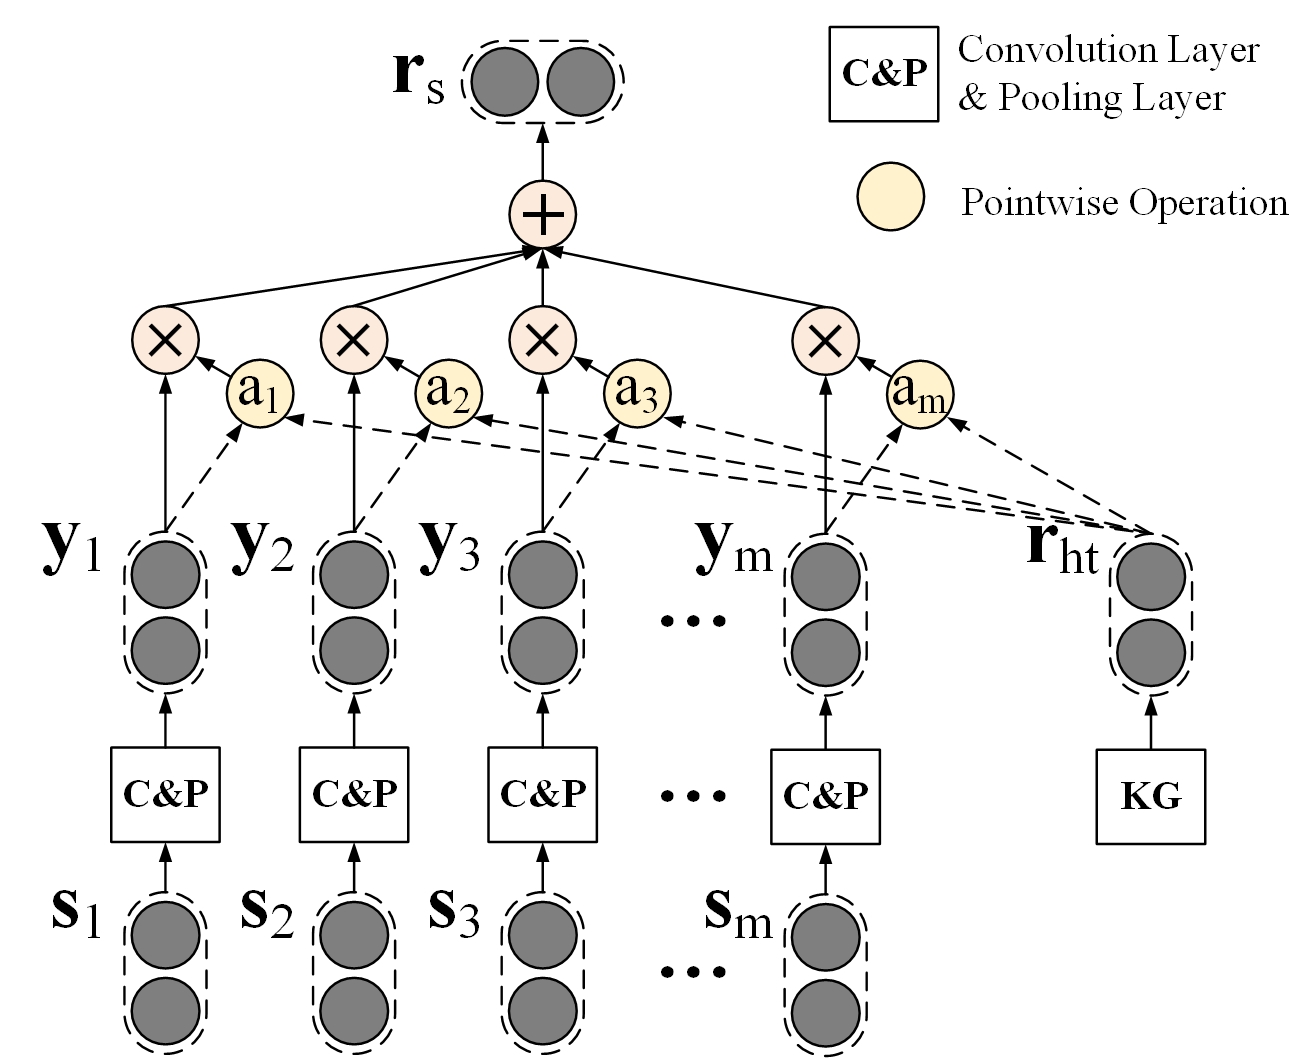
\includegraphics[width=0.9\columnwidth]{figures/ch3/cnn.jpg}
\caption{基于知识注意力机制的卷积神经网络模型}
\label{fig3:cnn}
\end{figure}

图\ref{fig3:cnn}描述了我们卷积神经网络的整个结构,也是文本关系表示学习模型的整个结构。对于任意一个标注了实体对$(h, t)$的句子$s$,如果实体对之间的关系为$r_s$的话,神经网络结构会以句子$s$的词语序列向量$\mathbf{s} = \{\mathbf{x}_1, \ldots, \mathbf{x}_n \}$作为输入。输入的句子向量在通过卷积神经网络中卷积与池化两层操作之后,输出一个文本意义描述的关系向量$\mathbf{y}$。由于存在多个句子标注了相同的实体,我们设置了一个基于知识图谱的注意力机制,用来在这些句子输出向量的基础上进行加权合并,然后得到一个全局的文本关系表示$\mathbf{r}_s$。对于句子的语义信息能在多大程度上描述文本关系,在经过一层多项逻辑斯特回归之后,我们用以下的能量函数来刻画:
\begin{equation}
\mathbf{o} = \mathbf{M}\mathbf{r}_s,
\label{eq3:cnn_distance}
\end{equation}
这里$\mathbf{M} \in \mathbb{R}^{\|R\| \times k_c} $是一个关系表示矩阵用来求得$\mathbf{r}_s$在不同关系上的能量评分,$k_c$是隐层向量的维度,最后我们可以定义一个条件概率$P((s, r_s)|{\theta_V})$:
\begin{equation}
P((s, r_s)|{\theta_V}) = \frac{\exp(\mathbf{o}_{r_s})}{\sum_{r \in R} \exp(\mathbf{o}_{r})}
\label{eq3:cnn_distance1}
\end{equation}

我们的文本关系表示模型就是由这几个部分构成的,包括输入层、卷积层、池化层、基于知识的注意力机制以及刚才介绍的分类层,相关细节将在下面一一展开。有了这些结构之后,我们衡量句子的语义能多大程度上表达某个特定关系就可以迎刃而解了。



\subsubsection{输入层}
 
给定一个含有$n$个单词的句子$s$,$s = \{ w_1, \ldots , w_n\}$,输入层的功能就是将$s$中的所有单词转化成对应的输入词向量$\mathbf{s} = \{ \mathbf{x}_1, \ldots , \mathbf{x}_n \}$。对于给定的句子$s$中任意一个单词$x_i$,其输入向量$\mathbf{x}_i$由两个实向量构成,一个是它的文本词向量$\mathbf{w}_i$,另一个是它的位置向量$\mathbf{p}_{i}$。

文本词向量可以将词的语义信息编码到低维空间中,并且通常会通过大量文本预先训练获得。大量的实验表明,以预先训练好的词向量作为网络输入可以有效提升神经网络的模型效果。在我们的工作中,词向量通过 Skip-Gram \cite{mikolov2013efficient}在大规模文本语料上提前训练获得。

位置向量的概念首次被提出是在 Zeng \cite{zeng2014relation} 的工作中。位置向量是一个可以表明给定单词与句子标注实体之间相隔距离的特征。举个例子,``\emph{马克吐温}出生于\emph{佛罗里达州}''中,\emph{马克吐温}与\emph{佛罗里达州}是标注出的实体,\emph{出}离\emph{马克吐温}和\emph{佛罗里达州}的距离分别为$1$和$-3$。我们会将这些距离也映射到维度$k_p$的连续空间上。对于句子$s$中给定的单词$w_i$,它的位置向量为$\mathbf{p}_i = [\mathbf{p}^h_i, \mathbf{p}^t_i]$, $\mathbf{p}^h_i, \mathbf{p}^t_i \in \mathbb{R}^{k_p}$,其中$\mathbf{p}^h_i$ 和 $\mathbf{p}^t_i$分别是到头实体以及尾实体之间的距离向量。

接着我们合并词向量$\mathbf{w}_i \in \mathbb{R}^{k_w} $与位置向量$\mathbf{p}_i \in \mathbb{R}^{k_p \times 2} $得到最终的输入向量$\mathbf{x}_i \in \mathbb{R}^{k_i} (k_i = k_w + k_p \times 2)$,从而卷积神经网络的输入为:
\begin{align}
\mathbf{s} & = \{\mathbf{x}_1,\ldots, \mathbf{x}_n\} \\\nonumber
&=\{[\mathbf{w}_1;\mathbf{p}_1],\ldots, [\mathbf{w}_n;\mathbf{p}_n]\}.
\end{align}




\subsection{卷积层}

卷积层将输入层得到的句子向量$\mathbf{s}$作为该层的输入,通过卷积层内的操作后导出为隐层向量$\mathbf{h}$。在卷积层中,我们在输入的序列向量$\mathbf{s}$上滑动一个尺寸为$m$的窗口。在每次窗口滑动中,我们可以采样得到一个局部的组合向量$\mathbf{\hat{x}}_i$:
\begin{equation}
\mathbf{\hat{x}}_i = \big[ \mathbf{x}_{i - \frac{m-1}{2}}; \ldots ; \mathbf{x}_i; \ldots ;\mathbf{x}_{i + \frac{m-1}{2}} \big],
\end{equation}
将输入序列$\mathbf{s}$落在以$\mathbf{x}_i$为中心的长度为$m$的窗口中的向量组合,就是这个组合向量$\mathbf{\hat{x}}_i$。如图\ref{fig3:conv_pooling}所示,如果窗口尺寸$m$为$3$,那么连续三个输入向量会组合成一个组合向量。然后,我们将这个组合向量$\mathbf{\hat{x}}_i$进行线性变换以及激活从而得到隐层向量$\mathbf{h}_i$
\begin{equation}
\mathbf{h}_i = \tanh(\mathbf{W}\mathbf{\hat{x}}_i + \mathbf{b}),
\end{equation}
这里,$\mathbf{W} \in \mathbb{R}^{k_c \times mk_i}$是卷积层的卷积核矩阵,$\mathbf{b} \in \mathbb{R}^{k_c}$是卷积层的偏移向量,$k_c$是隐层向量$\mathbf{h}_i$的维度。我们的激活函数选用了$\tanh$,激活的主要作用是将连续信号稳定约束在$[-1,1]$之间。

我们对一句话的理解不是割裂的,而是若干个语义小片段共同建立语义理解的,一个词如果不联系上下文是无法建立准确语义理解的。卷积层的主要物理意义就是在于对语言的局部语义采样,而窗口的大小就是上下文范围的大小。

\begin{figure}[h]
\centering
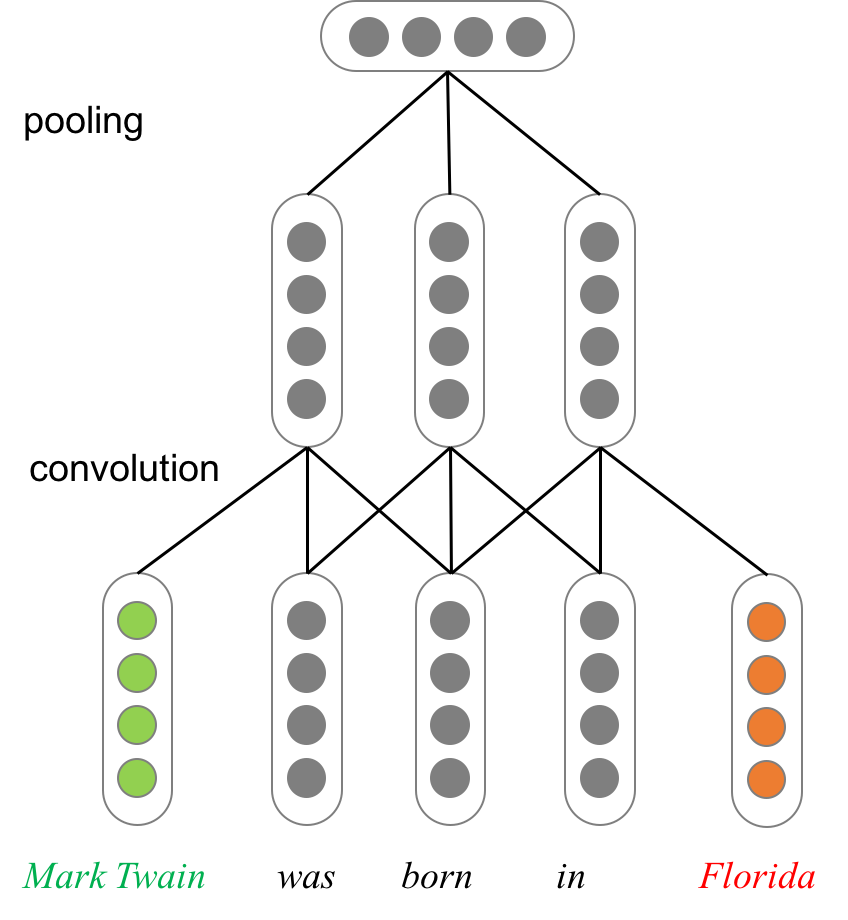
\includegraphics[width=0.7\columnwidth]{figures/ch3/cnn_concrete.png}
\caption{卷积层和池化层的结构示意图}
\label{fig3:conv_pooling}
\end{figure}



\subsection{池化层}

在池化层中,一个最大池化操作在隐层向量${\mathbf{h}_1, \ldots , \mathbf{h}_n}$上被实施,以便获得最后的输出向量$\mathbf{y} \in \mathbb{R}^{k_c} $,具体的过程如下:
\begin{equation}
\mathbf{y}_{j} = \max \{\mathbf{h}_{1,j}, \ldots, \mathbf{h}_{n,j} \},
\end{equation}
这里,$\mathbf{y}_{j}$是输出向量$\mathbf{y}$的第$j$维的值,$\mathbf{h}_{i,j}$是第$i$个隐向量$\mathbf{h}_i$的第$j$维的值。

池化层的主要作用在于对全局的特征进行汇总。在卷积层中,卷积实际上是对局部的语义进行特征提取。但是一个句子的语义仅仅依靠于局部特征是不恰当的,语义的理解最后还是要落实到全局的。池化的作用就是在每个局部采样输出的每个维度上选取一个信号最强值,从而最后能够汇总得到全局的语义特征,这是句子的语义理解中至关重要的一个步骤。如图\ref{fig3:conv_pooling}所示,所有的隐层向量池化输出一个整体的语义向量。

\subsection{基于知识的跨句注意力机制}

对于知识图谱中任意一个三元组$(h, r, t) \in T$,实际上可能存在若干个句子会包含这个三元组中的实体对$(h, t)$,并且这些句子的语义预示着实体对之间具有特定关系$r$。经过输入层、卷积层、池化层的操作后,这些句子已经有了输出向量${\mathbf{y}_1, \ldots , \mathbf{y}_m}$,$m$为包含这些实体对的句子数量。对于这些句子,我们认为其中的某些句子对最后的文本关系表示学习会更具有贡献性,所以我们需要一个机制来选取这些重要的句子同时规避大量句子带来的噪音。

在这里我们通过引入知识图谱中的潜在关系向量$\mathbf{r}_{ht} \in \mathbb{R}^{k_w} $来在神经网络中进行一个基于知识的注意力机制,从而强化重要句子的影响,具体形式如下:
\begin{equation}
\mathbf{e}_j  = \tanh(\mathbf{W}_s\mathbf{y}_j+\mathbf{b}_s)
\end{equation}
\begin{equation}
a_j  =\frac{\exp(\mathbf{r}_{ht}\cdot\mathbf{e}_j)}{\sum_{k = 1}^{m} \exp(\mathbf{r}_{ht}\cdot\mathbf{e}_k)}
\end{equation}
\begin{equation}
\mathbf{r}_s  = \sum_{j = 1}^{m} a_j\mathbf{y}_j
\end{equation}
这里,$\mathbf{W}_s \in \mathbb{R}^{k_w \times k_c}$是一个权重矩阵用来将前几层的输出向量转换到图谱空间中,$\mathbf{b}_s \in \mathbb{R}^{k_w}$则是线性变换的偏移向量。$a_j$是第$j$个句子输出向量$\mathbf{y}_j$在整个注意力机制结算后得到的权重评价。我们通过每个句子输出向量的权重来对这些向量进行加权求和从而得到一个全局的文本关系嵌入表示$\mathbf{r}_s$。有了全局的嵌入向量后,我们可以将向量$\mathbf{r}_s$带入式\ref{eq3:cnn_distance}以及式\ref{eq3:cnn_distance1}中进行分类。

\subsection{初始化及实现细节}
\label{sec3:detail}
在这一部分,我们主要介绍我们的模型在具体训练以及优化过程中的一些细节操作。对于我们以条件概率式\ref{eq3:topeq}为形式的任务目标,我们定义了一个对数似然函数来作为我们的优化目标,
\begin{align}
\mathcal{L}_{\theta}(G, D) & = \log P(G,D|{\theta}) + \lambda \lVert \theta \rVert_2 \\\nonumber
 & = \log P(G|{\theta_E, \theta_R}) + \log P(D|{\theta_V}) \\\nonumber
 & + \lambda \lVert \theta \rVert_2
\end{align}
这里,$\lambda$是一个超参,$\lVert \theta \rVert_2$是一个$L_2$距离的约束条件。我们的所有模型,包括 Prob-TransE 和 Prob-TransD 以及 CNN 都是通过随机梯度下降(stochastic gradient descent,SGD)算法来进行优化。值得注意的是,我们的损失函数的梯度会被传递到输入层的词向量上,因为这样才能将知识图谱的特征嵌入到词向量中。我们设计了一个多线程同步训练的模式来保障图谱和文本两方面的模型同时进行训练。每个线程控制一个模型以及所使用的训练数据。多个模型在内存上共用词、实体以及关系的嵌入表示,且不加锁,梯度则直接反馈到向量上而不考虑竞争问题。

\section{实验设计与结果分析}

我们提出的框架是一个涉及特征融合的联合学习框架,为了体现在框架下进行联合学习之后各个模型的效果提升,我们设计了两个不同任务的实验。第一个是知识图谱补全方向上的链接预测,第二个是文本关系抽取。在试验中,我们将图谱与文本模型联合学习,并将联合学习后的模型分别与各个经典算法进行对比来衡量特征融合的质量。

\subsection{实验设定}

\subsubsection{实验数据集}


\textbf{知识图谱。} 我们选用了 Freebase \cite{bollacker2008freebase} 来作为知识图谱这一块的数据来源。我们在引言中介绍过,Freebase 是一个被广泛利用的大规模知识图谱,并且对公众开放及提供数据下载。在我们的工作中,我们为实验环节引入了两个从 Freebase 中随机抽取的数据集合,包括 FB15K \footnote{https://everest.hds.utc.fr/doku.php?id=en:transe} 和 FB60K。FB15K 已经被很多工作采用并作为一个链接预测的标准测试集合长期存在。FB60K 是一个拓展自 Riedel \cite{riedel2010modeling} 发布的关系抽取文本的图谱数据集合,并且一直被用来进行作为关系抽取的标准数据。我们将 FB15K 和 FB60K 的数据集合详细细节罗列在表\ref{tab3:statistics-of-FB15K}中,包括实体数量、关系数量、事实三元组数量等等。

\begin{table}[htb]
\centering
\caption{FB15K 与 FB60K 的数据细节}
\begin{tabular}{|c|c|c|c|}
\hline
数据集合 & 关系 & 实体 & 三元组 \\ \hline
FB15K   & 1345           & 14951            & 592213 \\ \hline
FB60K   & 1324           & 69512            & 335350 \\ \hline
\end{tabular}
\label{tab3:statistics-of-FB15K}
\end{table}

\textbf{文本语料。} 我们从纽约时代周刊杂志(New York Times,NYT)的文章里选择合适的句子作为我们的文本语料。选取句子的方法是 Mintz \cite{mintz2009distant}提出的远距离监督算法(Distant Supervision),只要在一个句子里同时包含有一个三元组的头实体与尾实体,那么这个句子就会被加入我们的文本语料。我们提取了$194385$个同时包含有FB15K中头尾实体的句子,并且将句子标注为头尾实体所对应关系的正例。这些句子覆盖了FB15K中$47103$个事实三元组,共计$699$种关系以及$6053$个实体,我们将这个文本语料命名为 NYT-FB15K,即基于 FB15K 抽取的 NYT 文本语料。而 FB60K 的文本语料则是直接来自于 Riedel \cite{riedel2010modeling}在关系抽取中使用的数据,其中有$570088$个句子,覆盖了$63696$个实体,$56$种关系以及$293175$个事实三元组。我们将这个文本语料命名为 NYT-FB60K。

我们与之前的研究工作保持一致,FB15K 与 NYT-FB15K 用来在链接预测任务中进行评测,FB60K 和 NYT-FB60K 则被用在文本关系抽取这个任务上,这样的设定最大程度的保证了实验的公平性与可操作性。


\subsubsection{图谱文本匹配}
\label{sec3:alignment}

因为文本中的句子不是直接就含有实体标注以及实体关系标注的,所以我们不得不采用一些办法来标注句子中的实体以及实体的文本关系,从而能够支持我们联合学习框架的训练。具体的实施细节我们分为实体文本匹配以及关系文本匹配两个部分。


\textbf{实体文本匹配。}大量知识图谱中的实体出现在文本之中是一个很普遍的现象,而这也是我们试图融合图谱结构特征与文本语义特征的主要出发点。然而,将图谱中的实体与文本中的词相匹配却不是一件容易办到的事情。实体很准确,但是词却不是,一个词可能会指向多个不同的实体。举个例子,一个句子中的\emph{华盛顿},在不考虑上下文的情况下,可以指代美国国父也可以指代美国华盛顿特区。一个是人一个是地点,两者相去甚远。同样,\emph{苹果}可以是科技企业也可以是水果。在这里,我们使用了实体链接技术以及文本之间的锚链接来构建实体与词的匹配。由于文本的数据来源为网络资源,文章间的锚链接往往会指向一个实体,我们使用了这个信息将$E$的实体与词汇表$V$中的词匹配起来 \footnote{在我们的框架中,实体在$\theta_E$中的嵌入与对应词在$\theta_V$的嵌入在空间上是共享的。}。

\textbf{关系文本匹配。}正如我们在前文提到的那样,我们是可以从文本语料之中提取关系特征的。换句话说,关系的嵌入除了从图谱结构学习到之外也可以从文本语料中学习得到。受 Mintz \cite{mintz2009distant} 远距离监督算法的启发,我们也采用类似的方法来进行关系文本匹配。对于给定的一个关系$r \in R$,我们将所有存在关系$r$的实体对聚在一个集合中$Pair_{r} = \{(h, t) | (h, r, t) \in T \}$。然后,如果文本语料$D$中的某个句子同时包含有$Pair_{r}$中某个实体对的头尾实体,那么这句话将会被标注为关系$r$的正例。

\subsubsection{实验与模型参数设置}

在我们的联合框架中,我们从$\{0.1, 0.01, 0.001\}$之中为知识图谱$P(G|{\theta_E,\theta_R})$选择学习率$\alpha_k$,从$\{0.1, 0.01, 0.001\}$之中为文本模型$P(D|{\theta_V})$选择学习率$\alpha_t$。对于卷积神经网络的滑动窗口,我们从$\{3,5,7\}$之中选择滑动窗口的尺寸大小$m$。由于其它的一些参数对于实验影响不是非常大,并且出于实验背景统一与公平的考量,我们直接使用了过去一系列工作\cite{zeng2014relation,lin2016neural}对于卷积神经网络的参数设定。同样是为了与之前的相关工作进行对比,词、实体、关系的嵌入维度$k_w$在关系抽取任务中被设定为$50$,而在图谱填充的链接预测任务中,嵌入维度被设定为$100$。在表\ref{tab3:parameters}中我们罗列了实验中所有的参数细节。

\begin{table}[h]
\centering
\caption{联合学习框架参数设置}
\begin{tabular}{|cr|}
\hline
\multicolumn{1}{|c|}{约束系数 $\lambda$}                & 0.0001 \\
\multicolumn{1}{|c|}{知识图谱模型学习率 $\alpha_k$}        & 0.001 \\
\multicolumn{1}{|c|}{文本模型学习率 $\alpha_t$}             & 0.01  \\
\multicolumn{1}{|c|}{隐层向量维度 $k_c$}        & 230   \\
\multicolumn{1}{|c|}{词、实体、关系嵌入维度 $k_w$} & 50    \\
\multicolumn{1}{|c|}{位置向量维度 $k_p$}            & 5     \\
\multicolumn{1}{|c|}{窗口尺寸 $m$}    & 3     \\
\multicolumn{1}{|c|}{梯度传播中断概率 $p$}            & 0.5  \\
\hline
\end{tabular}
\label{tab3:parameters}
\end{table}



\subsection{关系抽取实验结果}

\subsubsection{测试结果}

在大量的工作中 \cite{mintz2009distant,riedel2010modeling,hoffmann2011knowledge,surdeanu2012multi,zeng2014relation,zeng2015distant,lin2016neural},文本模型都是用已有的知识图谱进行远距离监督,来自动地从文本中标注句子并加入到训练样例集合之中。从这些自动构建的训练数据中模型可以抽取语义特征并构建一个关系的分类器。我们也在这个机制上进行实验,以便评估联合学习对文本模型的效果提升。

我们采用了 Weston \cite{weston2013connecting}的实验设定来进行测试。严格意义上讲,关系抽取不是一个单分类任务,而是一个多分类任务。在测试过程中,对于测试实体对,我们会将所有的关系都作为候选与实体对进行计算。模型会给出每种关系在语义信息下与测试实体对的对应程度,并获得评分。一个关系,如果与实体对构成的三元组在知识图谱内,则为正确预测,反之为错误预测。测试系统会将评分进行排序,并且根据召回率与准确率的曲线来评估模型效果。

在 NYT-FB60K 数据集上的测试结果都被罗列在图\ref{fig3:jointcnn}中。图中``JointD+KATT''表示与 Prob-TransD 联合学习后具有知识导向注意力机制的卷积神经网络模型;``JointE+KATT''表示与 Prob-TransE 联合学习后具有知识导向注意力机制的卷积神经网络模型;``CNN+ONE''表示使用了 at-least-one 机制 \cite{zeng2015distant} 的卷积神经网络模型;``CNN+ATT''表示使用了句子级别注意力机制 \cite{lin2016neural} 的卷积神经网络模型,也是当前在关系抽取任务上效果最好的模型。除此以外,我们也将这一系列神经网络模型与经典的基于统计的关系抽取文本模型进行了对比,这些模型包括 Mintz \cite{mintz2009distant}、MultiR \cite{hoffmann2011knowledge}、MIML \cite{surdeanu2012multi} 以及 Sm2r \cite{weston2013connecting}。结果同样被罗列在图\ref{fig3:jointcnn}中。

\begin{figure}[h]
\centering
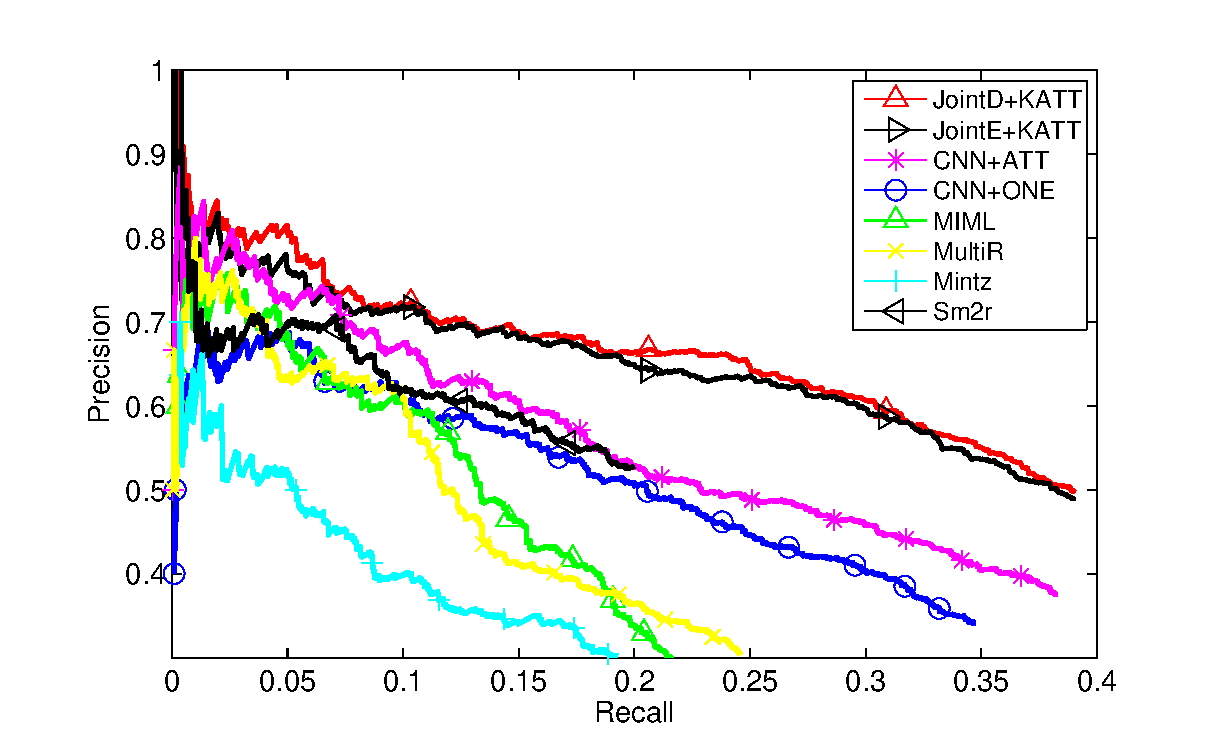
\includegraphics[width=1\columnwidth]{figures/ch3/res.eps}
\caption{JointD+KATT、JointE+KATT、CNN+ATT、CNN+ONE、MIML、MultiR、Mintz 与 Sm2r 的准确率/召回率曲线}
\label{fig3:jointcnn}
\end{figure} 

从实验结果中我们可以得出以下几个结论:

(1)与图\ref{fig3:jointcnn}中各个模型相比,经过联合学习框架训练之后的文本模型在整个召回率区间上都取得了最高的准确率,并且在效果上显著高出其余所有模型。当召回率大于$0.15$时,联合学习框架训练后的模型整体提升准确率在$10\%$到$20\%$之间。当召回率小于$0.15$时,模型也取得了最好的效果,并且比其余模型更为稳定。总的来说,联合学习模式下特征融合带来的受益在文本模型上体现的十分明显。

(2)除了 JointD+KATT、JointE+KATT 之外,CNN+ATT、CNN+ONE 与基于统计的模型相比,在召回率超过$0.15$的时候同样取得了超过$10\%$的准确率提升。并且整体上来看,神经网络模型准确率下降的速度要慢的多。这些实验结果很好的证明了深度神经网络没有局限在特征工程上,并且能够自行从原始数据中挖掘特征,稳定又有效。

(3)尽管基于统计的模型准确率都下降的非常快,尤其是与一系列神经网络模型相对比。但是在最高置信度的推荐中,即从$0$开始的一段召回率上,这些模型同样能够得到非常不错的准确率。这说明了,虽然人为设计的特征在某些方面存在局限性,但还是十分有效的。统计模型的主要优势在于其计算规模往往很小,且不需要过多的训练数据,但是有效特征需要人为构建与挑选。这些统计模型训练难度比基于神经网络的模型要简单的多,将两者进行结合并用于我们的工作,将是未来我们继续改进的一个重要方向。

\begin{table*}[h]
\centering
\caption{不同模型组合情况下的 P@N 评估结果(\%).}
\begin{tabular}{|c|ccc|ccc|} 
\hline
P@N(\%) & \multicolumn{3}{c|}{100}                                      & \multicolumn{3}{c|}{300} \\ \hline
& \multicolumn{1}{c|}{ONE} & \multicolumn{1}{c|}{ATT} & KATT & \multicolumn{1}{c|}{ONE} & \multicolumn{1}{c|}{ATT} & KATT \\ \hline
CNN+	& 67.3	& \textbf{76.2}	& -     & 58.1	& 59.8 	& -    \\ \cline{1-1}
JointE+  & 67.5 	& 74.1	& 75.8  & 63.0 	& 63.2 	& 68.0  \\ \cline{1-1}  
JointD+  & \textbf{68.5}    & 74.6  & \textbf{80.6}  & \textbf{67.0} & \textbf{67.3} & \textbf{68.7}  \\ \hline
P@N(\%) & \multicolumn{3}{c|}{500}                                      & \multicolumn{3}{c|}{Mean} \\ \hline 
& \multicolumn{1}{c|}{ONE} & \multicolumn{1}{c|}{ATT} & KATT & \multicolumn{1}{c|}{ONE} & \multicolumn{1}{c|}{ATT} & KATT \\ \hline
CNN+	& 43.7	& 48.5			& -     & 56.4 	& 61.5 	& -     \\ \cline{1-1}
JointE+  & 57.3 	& 59.3 	& 63.0  & 62.6 	& 65.5  & 68.9  \\ \cline{1-1}
JointD+  & \textbf{58.6}    & \textbf{61.1}  & \textbf{63.7}  & \textbf{64.8}   & \textbf{67.7}    & \textbf{71.0}  \\ \hline
\end{tabular}
\label{tab3:relationExt}
\end{table*}


\subsubsection{联合学习及基于知识的注意力机制的定量分析}

编码器至少一个机制(ONE),句子级注意(ATT)和我们基于知识的关注(KATT)。 “JointD”和“JointE”分别表示与Prob-TransD和Prob-TransE共同学习的CNN模型,“CNN”表示没有联合学习的CNN模型。 结果显示在表\ ref {tab3:relationExt}中,包括P @ 100,P @ 200,P @ 300及其平均值。

对于关系抽取,我们通常会更加注意那些具有最高置信度得分的推荐。毕竟我们并不指望模型能够达到十全十美,高置信度的推荐保持一个很好准确率其实更符合我们的应用需求。为了能够更详细地比较联合学习前后模型结果上的变化,我们采用了另一种评估推荐效果的测试方式。我们将推荐得分排序后,选取最高置信度的若干个推荐,此时预测的准确率将作为我们衡量模型能力的指标。

在这个实验中,我们选择 Zeng \cite{zeng2014relation} 使用过的卷积神经网络作为文本编码的模型。卷积神经网络编码器将会与不同种类的跨句学习机制相结合,包括 at-least-one 机制(ONE),句子级别注意力机制(ATT)以及我们的基于知识的注意力机制(KATT)。这样的组合可以对各个跨句合并机制进行定量分析。

我们也将文本模型与知识图谱表示学习模型相结合,从而定量分析联合学习带来的影响。``JointD''表示与 Prob-TransD 联合学习之后卷积神经网络得到的文本模型,``JointE''表示与 Prob-TransE 联合学习之后卷积神经网络得到的文本模型,``CNN''表示没有与知识图谱进行联合学习的卷积神经网络文本模型。具体各种组合的效果被罗列在表\ref{tab3:relationExt}中,包括前$100$推荐准确率P@100、 前$300$推荐准确率P@300、前$500$推荐准确率P@500以及准确率的平均值。

从实验结果我们可以得出以下几点:

(1)所有的文本编码器,无论是采用哪种跨句学习机制,在联合学习框架下进行训练之后,都在效果上有大幅度的提升。从平均的推荐准确率来看,联合学习后 CNN+ONE 的准确率提升了$6\%$左右,而 CNN+ATT 的准确率也提升了$5\%$左右。实验结果表明,我们提出的平行联合学习框架在效率提升之外,特征融合也得到了保障,联合学习后文本模型接收到图谱的影响提升了自身的推荐效果。


(2)比起与Prob-TransE进行联合学习的文本编码器,与Prob-TransD进行联合学习的文本编码器进一步提升了推荐效果。Prob-TransD是一个比Prob-TransE更复杂,更具有表达能力的知识图谱表示学习模型,并且可以更好地提取知识图谱特征以及理解实体之间关系的多样性。毕竟,在Prob-TransD中,实体在不同关系的环境下是具有不同的嵌入的,这可以更好地满足图谱中多样性的表达需求。实验结果也表明,联合学习框架可以利用图谱辅助训练文本模型,并且对图谱模型的适应性很好。图谱模型的效果也影响特征融合的效果,表达能力越强的图谱模型对文本模型的效果提升越明显。

(3)在表\ref{tab3:relationExt}中,注意力式的跨句合并机制 ATT、KATT 比单纯的 ONE 机制要有效的多。训练过程中所使用的文本语料是基于远距离监督机制自动抓取构建的,在构建过程中会引入大量杂质和噪音。这很好理解,一个实体对如果出现在一个句子中,这个句子很有可能在语义上无法描述实体间的关系。而注意力机制能够获取到最有意义的句子并从这个句子里学到更有意义的嵌入,所以在效果上比简单的特征合并要高出许多。


(4)ATT 和 KATT 的比较进一步表明,在跨句合并机制上,不使用知识图谱信息的简单注意力机制还是略显薄弱的。即使是含有相同关系的不同实体对,实体间的关系都有着细微的差别,这与我们在前文提到的实体多样性以及关系多样性有关。ATT 中通过一个模糊的全局向量来进行重要的句子选择,显然这是无法满足关系多样性的特性的。在这里,我们将知识图谱的信息融入到注意力机制中。对于不同的实体对,我们给出局部的向量来进行重点句子选择,而这些局部向量在全局上又密切相关。因此,我们基于知识的注意力机制比直接跨句的简单注意力机制更具有区分度与甄别能力。

\subsection{图谱填充实验结果}

针对实体的链接预测被广泛地使用在知识图谱填充任务中\cite{bordes2013translating,wang2014transh,lin2015learning}。在这里,我们的任务设置和章节\ref{cha2:framework}中链接预测是一致的,给定一个头实体和关系的组合$(h, r, ?)$来预测对应的尾实体,或者给定一个尾实体和关系的组合$(?, r ,t)$。

对于每个测试的三元组$(h,r,t)$,我们用FB15K中的所有实体来替换头实体或者尾实体,按照公式\ref{eq3:kg_distance}计算出评分后以降序排列。依照我们对模型的设想,事实三元组$(h,r,t)$如果成立的话,其对应的评分应当比替换后所有的三元组都要高。我们遵循以往工作一贯的设定,使用正确实体能量得分排在前十的比例来衡量预测质量,我们将这个结果称为$10$预测命中率(Hits@10)。

Bordes\cite{bordes2013translating} 在其工作中将知识图谱中的关系划分为四个大类:一对一(1-to-1)、一对多(1-to-N),多对一(N-to-1)、多对多(N-to-N)。实验也在这四类关系上分别进行了测试与分析。我们同样汇报了不同关系类别上的 Hits@10 结果,包括头实体预测、尾实体预测两个任务方向。除此以外,我们汇报了三元组级别的平均准确率用以刻画模型整体的效果。

由于实验的设定是相同的,所以我们直接从相关工作\cite{bordes2011learning,bordes2012joint,bordes2013translating,wang2014transh,lin2015learning,ji2015knowledge}中引用了 SE、SME、TransE、TransH、TransR、CTransR、TransD 在 FB15K上的实验结果。我们自己动手实现了 TransD,并使用 Github 上 KB2E\footnote{https://github.com/thunlp/KB2E}工具包来实现其他的一些图谱模型。在我们的框架中,没有进行联合学习的知识表示模型被称为``Prob-TransE''和``Prob-TransD'',与卷积神经网络文本模型一起进行联合学习的知识表示模型被命名为``JointE''和``JointD''。具体实验结果显示在表\ref{tab3:entity}之中。

为了进一步论证我们联合框架的有效性,我们也通过关系级别的平均 Hits@10 准确率来刻画模型整体的效果。在关系级别的平均准确率上,Prob-TransE 与 JointE 的结果分别为$\textbf{66.2\%}$和$\textbf{80.4\%}$。Prob-TransD 和 JointD 的结果分别为$\textbf{71.4\%}$和$\textbf{85.1\%}$。


\begin{table*}[h]
\centering
\caption{头尾实体链接预测的结果(\%).}
\scalebox{0.90}{
\begin{tabular}{|c|cccc|cccc|c|}
\hline
度量方法            & \multicolumn{4}{c|}{Predicting Head} & \multicolumn{4}{c|}{Predicting Tail} & \multicolumn{1}{c|}{Overall} \\ \hline
类别  & 1-to-1     & 1-to-N    & N-to-1    & N-to-N    & 1-to-1     & 1-to-N    & N-to-1    & N-to-N  & Triple Avg. \\ \hline

SE \cite{bordes2011learning}&35.6 &62.6 &17.2 &37.5 &34.9 &14.6 &68.3 &41.3 &39.8  \\ 
SME \cite{bordes2012joint}&35.1 &69.6 &19.9 &40.3 &32.7 &14.9 &76.0 &43.3 &41.3  \\ 
TransE \cite{bordes2013translating}            & 43.7       & 65.7      & 18.2      & 47.2      & 43.7       & 19.7      & 66.7      & 50.0    & 47.1  \\ 
TransH \cite{wang2014transh}    & 66.8       & 87.6      & 30.2      & 64.5      & 65.5       & 39.8      &83.3      & 67.2    & 64.4  \\ 
TransR \cite{lin2015learning}   & 78.8       & 89.2      & 38.1      & 66.9      & 79.2       & 38.4      &90.4      & 72.1    & 68.7  \\ 
CTransR \cite{lin2015learning}    & 81.5      & 89.0      & 36.4      & 71.2      & 80.8       & 38.6      &90.1      & 73.8    & 70.2  \\ 

TransD \cite{ji2015knowledge} &81.2  &94.8  &47.1 &79.3  &81.6 &53.9 &93.7 &82.5  &78.9  \\ \hline


Prob-TransE      & 66.5       & 88.8      & 39.8      & 79.0      & 66.4       & 51.9      & 85.6      & 81.5    & 76.6  \\
JointE     &82.7 & \textbf{96.2} &45.0 &80.7 &81.7& 57.7 & 93.6 &84.0 & 79.3  \\ \hline

Prob-TransD		&79.1	&93.0 &42.2	&79.2	&79.2	&51.6	&90.9	&82.7	&78.2  \\  

JointD    &\textbf{82.7}   &95.2 &\textbf{47.8} & \textbf{81.6} &\textbf{82.0} &\textbf{57.9} & \textbf{94.7} &\textbf{84.7} & \textbf{80.4}  \\ \hline
\end{tabular}}
\label{tab3:entity}
\end{table*}


从实验结果我们可以观察到以下几点:

(1)无论是预测头实体,还是尾实体,联合学习框架下的图谱模型在四大类关系上几乎都得到了的改善。特别是,Joint-TransE 与 Joint-TransD 比起 Prob-TransE 和 Prob-TransD,在关系级别的平均准确率上实现了超过$10\%$的提升。这表明,联合学习之后对知识图谱嵌入表示带来的提升是一致且鲁棒的,并且在框架下与文本模型一起学习的知识图谱表示模型可以很好的利用文本语义与文本关系的对应来提升关系层次的表达能力。

(2)与多对多的关系相比,一对一、一对多以及多对一关系上,联合学习框架下学习得到的模型提升效果更为明显。这表明我们联合学习框架融入的文本特征,对确定性关系的嵌入有很好的帮助。在数据集合 FB15K 中,超过$80\%$的三元组属于多对多关系的实例。由于联合学习模型在多对多关系上的效果提升没有其他类别关系上显著,因此在三元组级别的平均准确率上,提升没有关系级别的平均准确率突出。

(3)TransD 是 TransE 的扩展的模型,具有更复杂的实体嵌入机制。在 TransD 中,每个实体在不同的关系空间中具有不同的嵌入表示。与其他的模型相比,TransD 可以取得更好的实验结果。而在联合学习框架中与文本模型一起学习后,TransD 进一步提高了效果。这些结果意味着与 TransE 和 TransD 相似的其他知识图谱表示学习模型,如 TransH、TransR 等,都可以用类似的方法与我们的框架进行整合。

\section{本章小结}

在本章节中,我们提出了一个通用的联合学习框架来将知识图谱与文本模型进行结合。我们的联合学习框架将实体、关系和文本词汇嵌入到统一的连续空间中,并通过这样的方式来进行特征融合。更进一步,我们采用了图谱文本匹配以及基于知识的注意力机制来交换知识图谱模型与文本模型之间的信息。值得注意的是,以往的模型多是串行结合的模式,而我们采用了并行结合的模式以便在训练效率上有大幅度提升。在实验阶段,我们使用关系抽取来度量文本模型,使用链接预测来度量图谱模型。实验结果表明,我们平行的联合学习框架可以有效学习知识图谱与文本的嵌入表示,并且得到的嵌入更具有区分性与辨识度。通过结合不同的知识图谱表示学习模型,我们证明了联合框架对现有图谱模型的开放性,不同的图谱模型都可以被吸收进入框架。在未来的工作中,我们将尝试使用高效的实现方式来将循环神经网络 RNN 用作文本编码器。与统计模型相结合以及融入更多的特征作为联合框架的指导,比如图谱的关系路径、文本的语法关联,也是非常有意义的尝试方向。








\chapter{结论与展望}
\label{cha:conclusion}

\section{结论}




知识图谱是将人类已有知识高度结构化形成的知识系统,凝结了人类千百年 积累的知识与智慧。知识图谱常被用于信息检索、问答系统和智能对话等知识驱 动的人工智能应用,辅助知识抽取、存储与推理,具有重要的实用价值与研究意 义。随着互联网时代信息的爆炸性增长,如何对知识图谱中存储的知识进行更好 地编码与表示,构建知识图谱到知识驱动的应用之间的桥梁,成为当下热门的研 究课题。为了解决计算效率与数据稀疏等问题,知识表示学习应运而生,它基于分 布式表示的思想,将实体和关系的语义信息在低维向量空间中进行表示,显著提 高了知识表示的灵活性和性能。现在,知识的分布式表示已被广泛运用于关系抽 取[58]、语言模型[59] 和问答系统[60] 等知识驱动的任务中。



\section{存在的问题与改进思路}

\section{未来的工作}







我们身处于复杂多元的世界,每时每刻都需要与各种多源信息,如文本、图 像和结构化信息等多模态信息进行交互。这些多源信息既是我们不可或缺的知识 来源,亦是我们反馈自身信息的对象与媒介。然而,传统的知识表示学习模型往 往重点关注知识图谱自身的高度结构化信息,忽略了丰富的跨模态多源信息。在 本文中,我们主要关注融合多源信息的知识表示学习,其中重点关注以下三个任 务:(1)融合实体描述信息的知识表示学习;(2)融合实体层次类型信息的知识 表示学习;(3)融合实体图像信息的知识表示学习。
在第二章,我们重点关注融合实体描述信息的知识表示学习。实体描述是对 实体自身凝练的文本描述,其中蕴含着实体各方面的丰富细节信息。这些文本信 息能够作为知识图谱结构化信息的补充,帮助构建更准确的知识表示。然而,联合 考虑实体描述面临着如何自动抽取描述中高质量的文本信息,以及如何融合结构 信息与文本信息进行联合学习等挑战,已有引入文本信息的知识表示模型也仅仅 孤立地考虑词级别的文本信息,而忽略了篇章级别语序语义信息的影响。为了解 决这些问题,我们基于平移假设提出了融合实体描述的知识表示学习模型,为每 个实体设置了基于结构与基于描述的两种表示,并使用神经网络模型对实体描述 进行建模。实验结果表明,我们的模型能够充分利用实体描述中的文本信息,提升 知识图谱补全和实体类型分类等任务的效果,在对新实体的知识表示上也有较好 的表现。
在第三章,我们重点关注融合实体层次类型信息的知识表示学习。实体层次 类型指的是实体所属不同粒度的类型信息,这些类型往往储存在层次化的结构中。
63
第 5 章 总结与展望
 实体类型信息能够帮助人类构建层次化的认知体系,提供实体结构化的先验知识, 也能暗示实体在不同情境下更应表现出的类型。然而,传统知识表示模型较少考 虑实体类型信息,也未能充分利用实体类型的层次结构信息。为了解决这些问题, 我们设计了融合实体层次类型的知识表示学习模型,提出实体在不同关系下应该 突出不同实体类型,并具有类型特化的实体表示。我们使用两种层次类型编码器 对实体类型的层次结构进行建模,构建映射矩阵,同时在训练与测试中进行了实 体类型限制,进一步提高知识表示的性能。实验结果表明,我们的模型能够充分利 用实体层次结构的类型信息,提升知识图谱补全和三元组分类等任务的效果,并 在长尾分布的数据集上也能得到超过基线模型的表现。
在第四章,我们重点关注融合实体图像信息的知识表示学习。实体图像能够 提供实体外形、行为和其它相关实体的视觉信息,可以帮助模型全方位地理解实 体。融合图像信息与知识图谱结构信息构建跨模态的知识表示,既能通过图像信 息提高知识表示的性能,也能将知识引入图像领域,为图像与知识的联合应用提 供基础。由于图像信息与知识信息在储存与表示上存在较大差异,如何联合两个 异质空间进行学习成为此任务的最大的挑战。另外,海量的图像信息质量良莠不 齐,选取的图像质量对知识表示结果也有较大影响。针对这些问题,我们提出了融 合实体图像的知识表示学习模型,构建实体基于描述和基于图像的两种知识表示。 具体地,我们使用基于神经网络模型的图像表示模块和图像映射模块构建图像特 征在知识空间的表示,然后引入注意力机制自动选择高质量的实体图像构建实体 基于图像的表示。实验结果证实了实体图像中的视觉信息能够帮助模型构建更准 确的知识表示,在知识图谱补全和三元组分类等任务上都表现出更好的效果。经 过实例分析,我们也证实了模型在图像-知识联合空间上的语义平移现象,以及注 意力机制对模型效果的正面影响。


%%% 其它部分
\backmatter

%% 本科生要这几个索引,研究生不要。选择性留下。
% 插图索引
\listoffigures
% 表格索引
\listoftables
% 公式索引
\listofequations


%% 参考文献
% 注意:至少需要引用一篇参考文献,否则下面两行可能引起编译错误。
% 如果不需要参考文献,请将下面两行删除或注释掉。
\bibliographystyle{thuthesis}
\bibliography{ref/refs}


%% 致谢
% 如果使用声明扫描页,将可选参数指定为扫描后的 PDF 文件名,例如:
% \begin{acknowledgement}[scan-statement.pdf]
\begin{acknowledgement}

衷心感谢我的指导老师刘知远助理教授对我的精心指导。在本科的四年里,他为我创造了良好的学术氛围、优越的科研环境以及优质的学术交流机会。他循循善诱,引导我在自然语言处理领域不断探索,言传身教使我深受启发且受益良多。

感谢清华大学自然语言处理组林衍凯、谢若冰学长为代表的诸多前辈在科研工作中给予我的交流、探讨和帮助,尤其是在进组之初的答疑解惑,确定研究方向之后的论证建议,投稿论文时的严格把关,让我在学术道路上不再孤单。

感谢清华大学计算机科学与技术系的诸多老师们多年来的悉心教导,在专业课程上给予我充分锻炼,在课程外给予我充分拓展,使我能够对专业有着全局性的视野和把握,也让我在这四年中个人能力得到了巨大锻炼。

感谢大学期间我的朋友们给我的关心和陪伴,无论是班级同学、思源十三期的同学还是实验室同届的同学,和大家在一起的日子我十分的快乐和满足。无论是远赴海外的吴佳炜、徐磊、曾文远同学,还是和我继续留在实验室的郭志芃同学,祝大家都将有一个美好的人生,有缘再聚。

最后我要感谢我的家人。在我走来的一路上,你们一直是我的坚固堡垒和强力后盾,在后方给予我无限的支持,让我能够无所畏惧的向前冲刺。
在参与信息竞赛的道路上,尤其是低谷之时,你们始终给我鼓励与支持,让我有无限勇气来坚持到底。对于即将参与高考的表弟和堂妹,我也衷心祝愿你们取得优异成绩,努力把握自己的人生。

\end{acknowledgement}


%% 附录
\begin{appendix}
\chapter{外文资料的调研阅读报告或书面翻译}

\title{知识图谱填充任务中实体与关系的表示学习}

{\heiti 摘要:} 

知识图谱填充是一个预测知识图谱实体间链接关系类型的任务。在本篇论文中,我们提出了一个知识图谱嵌入的算法来解决这个问题。在最近的研究中,诸如 TransE 和 TransR 这样的模型将关系作为头实体到尾实体之间的转移来对知识图谱进行嵌入。通常,这类算法会将实体和关系在同一个连续空间中进行嵌入。实际上,一个实体可能有多个方面,即在不同关系下拥有不同的意义,这使得在一个统一的空间中建模变的很困难。在本文中,我们提出了叫作 TransR 的模型来将实体和关系在不同空间中嵌入。然后,在这个模型中我们再学习实体空间和关系空间的映射关系,从而将实体从实体空间映射到关系空间中来构建头实体到尾实体之间的转移。在试验中,我们在三个任务上评测了我们的模型,包括链接预测,三元组分类和关系现实抽取。实验结果和之前最好的模型相比有显著的提升,这些模型中包括 TransE 和 TransH。这篇论文的源代码被我们公布在 https://github.com/mrlyk423/relation\_extractio 上。

\section{引言}

  \begin{figure}[htb]
  \centering
  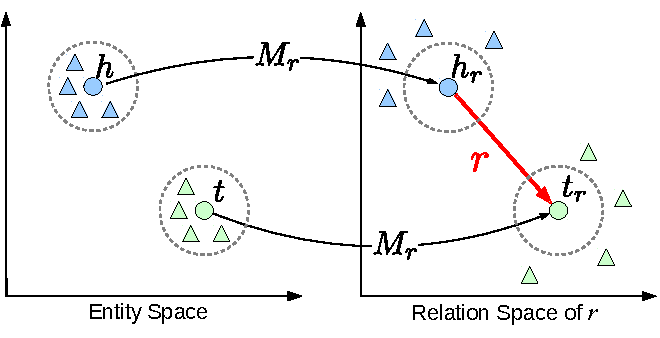
\includegraphics[width=0.8\columnwidth]{figures/trans/model_idea}
  \caption{Simple illustration of TransR.}
  \label{fig_1:idea}
  \end{figure}

知识图谱可以将实体和实体间丰富的关系信息进行结构化。尽管一个经典的知识图谱可能含有数百万个实体和数以亿个关系事实,这个图谱离完善还差的很远。知识图谱填充这个任务就是为了在已有图谱信息的监督下进行学习并能够预测实体间的未知关系。这个任务可以推理出新的关系事实,从而也对从自由文本中进行关系抽取有很重要的作用。

知识图谱填充和社交网络中的链接预测非常相似,但是更具有挑战性,主要原因有以下几点:(1)知识图谱中的节点代表的实体通常具有不同的关系与属性;(2)知识图谱中的边代表的关系也是有不同类型的。对于知识图谱填充,我们不仅需要知道实体之间是否有关系还要知道这个关系是哪种具体的类型。

因为这个原因,传统的用来做链接预测的方法对于图谱填充是不适用的。最近,一个极有发展潜力的模型被提出用来将知识图谱嵌入到一个连续的向量空间中同时在空间中保持图的特性。紧跟着这个工作,大量的方法被尝试和提出,这个我们将会在``相关工作''章节细节阐述。

在这些方法中,TransE \cite{bordes2013translating} 和 TransH \cite{wang2014knowledge} 最为简洁有效,并且取得了最好的预测效果。受 \cite{mikolov2013distributed} 的启发,TransE 将实体和关系都嵌入为空间中的向量。这些向量的维度为 $\mathbb{R}^k$,我们也用加粗的符号来代表对应的向量。Trans 最基本的想法就是将实体之间的关系对应到实体向量间的转移,即知识图谱中的三元组$(h, r, t)$,我们有$\mathbf{h} + \mathbf{r} \approx \mathbf{t}$。因为 TransE 对于 1-to-N、N-to-1、N-to-N 的关系建模有一定的问题,TransH 被提出以便将实体在不同的关系下拥有不同的表示从而适应这种非一对一的关系。

无论是 TransE 还是 TransH 都将实体和关系嵌入到同一个$\mathbb{R}^k$的空间中去。但是,我们之前说到的,一个实体在不同的关系下是有所区别的。因此,有这样一个显而易见的现象,相似的实体会在空间上非常接近,但是在不同的关系背景下我们又希望它们有区分性,即距离上要相互远离,这两者在同一个空间中是矛盾的。为了解决这个问题,我们提出了一个新的方法,将实体和关系在各自的空间中进行嵌入,例如实体在一个实体空间中,不同类型的关系在不同的关系空间中,并且要构建一个映射机制能够将实体从实体空间映射到不同的关系空间中去,我们将这个方法命名为 TransR。

TransR 的基础想法如图\ref{fig_1:idea}所示。对于一个给定的三元组$(h, r, t)$,实体首先从实体空间被映射到关系$r$所在的关系空间中去成为$h_r$和$t_r$,映射为$M_r$,然后有$\mathbf{h}_r + \mathbf{r} \approx \mathbf{t}_r$。通过这样的一种映射,我们可以使得头尾实体能够在空间中具有相似性,而在不同的关系中又有不同的空间表现。

更进一步,即使在同一个类型的关系下,实体间的潜在关联也是具有多样性的。所以即使对于每一个关系都构建一个向量也是不够的。举个例子,头尾之间的关系``行政区划覆盖''可能具有很多中关系模式,比如``国家-城市''、``国家-大学''、``洲-国家''等等。受到分段线性回归 \cite{ritzema1994drainage} 的启发,我们通过将头尾实体间的潜在关系进行聚类,并为每一个聚类的簇单独建立向量表示的方法进一步拓展了TransR,并且命名为 CTransR。
 
我们在三个任务上评测了我们的模型,包括链接预测,三元组分类和关系现实抽取,数据也是从WordNet和Freebase中抽取出专门用来做性能评测的标准数据集。实验结果和之前最好的模型相比有显著的提升,体现了我们模型的有效性。

\section{相关工作}

    \subsection{TransE和TransH}

    正如我们在``引言''中介绍的那样,TransE \cite{bordes2013translating} 希望图谱中的三元组$(h, r, t)$满足$\mathbf{h} + \mathbf{r} \approx \mathbf{t}$。这表明$(\mathbf{t})$在空间中应该是最接近$(\mathbf{h} + \mathbf{r})$的。因此,TransE 定义了这样一个评分函数:
    \begin{equation}
    f_{r}(h, t) = \|\mathbf{h} + \mathbf{r} - \mathbf{t}\|_{2}^{2},
    \end{equation}
    函数值越低代表$(h, r, t)$存在的可能性越大,反之亦然。

    TransE 在 1-to-1 的关系上表现突出,但是在 N-to-1, 1-to-N 以及 N-to-N 这些类别的关系上存在问题。我们以一个 1-to-N 类别的关系$r$作为案例。$\forall i \in \{0, \ldots, m\}, (h_i, r, t) \in S$. 这表明$\mathbf{h}_0 = \ldots = \mathbf{h}_m$,然而这和实际现象是违背的。

    为了解决TransE在 N-to-1, 1-to-N 以及 N-to-N 类别关系上的问题,TransH \cite{wang2014knowledge} 被提了出来,并用以将实体在不同关系的环境下嵌入不同的分布式表示向量里去。对于任意的关系$r$,TransH 将关系建模为一个法向量为$\mathbf{w}_r$的超平面上的向量$\mathbf{r}$。对于任意一个三元组$(h, r, t)$,



    实体的向量$\mathbf{h}$和$\mathbf{t}$首先被映射到$\mathbf{w}_r$的超平面上成为$\mathbf{h}_{\bot}$和$\mathbf{t}_{\bot}$,接着和TransE类似的定义出评分函数:
    \begin{equation}
    f_{r}(h, t) = \|\mathbf{h}_{\bot} + \mathbf{r} - \mathbf{t}_{\bot}\|_{2}^{2}。
    \end{equation}
    在$\|\mathbf{w}_r\|_{2} = 1$的约束下, 参数满足$\mathbf{h}_{\bot} = \mathbf{h} - \mathbf{w}_{r}^{\top}\mathbf{h}\mathbf{w}_{r}$,以及$\mathbf{t}_{\bot} = \mathbf{t} - \mathbf{w}_{r}^{\top}\mathbf{t}\mathbf{w}_{r}$。正是通过将实体向量映射到关系超平面上,我们使得实体在不同的关系环境下有不同的表示。


    \subsection{其他模型}
    除了 TransE 和 TransH,还有许多其他模型可以用来对知识图谱进行嵌入。这里我们介绍一些经典的模型方案,并且也会作为我们的实验对比在实验环节体现。

    \textbf{Unstructured Model (UM)。} UM \cite{bordes2012joint,bordes2014semantic} 是一个简化版本的 TransE,即在 TransE 的基础上满足$\mathbf{r} = \mathbf{0}$, 此时我们的评分函数为$f_r(h, t) =  \|\mathbf{h} - \mathbf{t}\|_{2}^{2}$。很显然,这个模型无法处理实体间多种关系的情况。

    \textbf{Structured Embedding (SE)。} SE \cite{bordes2011learning} 为头实体和尾实体设计了不同的变换矩阵,比如$\mathbf{M}_{r, 1}$和$\mathbf{M}_{r, 2}$,并且在这些变换矩阵的基础上定义了$L_1$距离的评分函数,$f_r(h, t) =  \| \mathbf{M}_{r, 1} \mathbf{h} - \mathbf{M}_{r, 2} \mathbf{t} \|_1$。由于模型具有两个独立的变换矩阵,因此不能捕获实体和关系之间的精确关系。

    \textbf{Single Layer Model (SLM)。} SLM 是 NTN \cite{socher2013reasoning}的简化版本。评分函数如下:
    \begin{equation}
    f_{r}(h, t) = \mathbf{u}_r^\top g (\mathbf{M}_{r, 1} \mathbf{h} + \mathbf{M}_{r, 2} \mathbf{t}),
    \end{equation}
    这里$\mathbf{M}_{r, 1}$和$\mathbf{M}_{r, 2}$是权重矩阵,$g()$是\texttt{tanh}操作。SLM 是 NTN 在张量被设置为$\mathbf{0}$时的特例。


    \textbf{Semantic Matching Energy (SME)。} SME \cite{bordes2012joint,bordes2014semantic} 可以通过多重矩阵乘法和哈达玛积来获取实体和关系之间的相关性。SME 模型将关系表示为一个独立的向量,这些向量通过线性矩阵乘积与实体向量相互作用,并且关系向量内部共享相同的参数。SME 定义了两个语义能量函数用于优化,包括线性形式:
    \begin{equation}
    f_r(h, t) = (\mathbf{M}_{1} \mathbf{h} + \mathbf{M}_{2} \mathbf{r} + \mathbf{b}_1 )^{\top} (\mathbf{M}_{3} \mathbf{t} + \mathbf{M}_{4} \mathbf{r} + \mathbf{b}_2),
    \end{equation}
    和双线性形式:
    \begin{equation}
    f_r(h, t) = \big( (\mathbf{M}_{1} \mathbf{h}) \otimes (\mathbf{M}_{2} \mathbf{r}) + \mathbf{b}_1 \big)^{\top} \big( (\mathbf{M}_{3} \mathbf{t}) \otimes (\mathbf{M}_{4} \mathbf{r}) + \mathbf{b}_2 \big),
    \end{equation}
    这里$\mathbf{M}_{1}$,$\mathbf{M}_{2}$,$\mathbf{M}_{3}$和$\mathbf{M}_{4}$是权重矩阵,$\otimes$是哈达玛积,$\mathbf{b}_1$和$\mathbf{b}_2$是线性偏置向量。在 \cite{bordes2014semantic}的工作中,SME 的双线性形式被重新定义为三路张量而不是矩阵。

    \textbf{Latent Factor Model (LFM)。} LFM \cite{jenatton2012latent,sutskever2009modelling} 考虑使用实体嵌入之间的二阶相关性来定义一个双线性评分函数$f_r(h, t) = \mathbf{h}^{\top}\mathbf{M}_r\mathbf{t}$。

    \textbf{Neural Tensor Network (NTN)。} NTN \cite{socher2013reasoning} 定义了一个表达能力很强的评分函数:
    \begin{equation}
    f_{r}(h, t) = \mathbf{u}_r^\top g (\mathbf{h}^{\top} \mathbf{M}_r \mathbf{t} + \mathbf{M}_{r, 1} \mathbf{h} + \mathbf{M}_{r, 2}\mathbf{t} + \mathbf{b}_r),
    \end{equation}
    这里$\mathbf{u}_r$是一个针对关系的线性变换层,$g()$是\texttt{tanh}操作,$\mathbf{M}_r \in \mathbb{R}^{d \times d \times k}$是一个三路的张量,$\mathbf{M}_{r, 1}, \mathbf{M}_{r, 2} \in  \mathbb{R}^{k\times d}$则是权重矩阵。在表达能力强的同时,NTN 的高复杂度使得它很难在大规模知识图谱上被应用。

    考虑到时间问题,在实验部分我们将会和\textbf{RESCAL}, 一个 \cite{nickel2011three,nickel2012factorizing} 提出的类似的矩阵分解算法来对比。


    \section{我们的模型}
    \label{sec:method}

    为了解决 TransE 和 TransH 在表示学习中的一些问题,我们提出了 TransR ,该模型可以将实体和关系在不同的空间中进行嵌入,并且通过特殊的矩阵将实体映射到关系空间中。

    \subsection{TransR}


    TransE 和 TransH 都将实体和关系嵌入到相同的维度为$\mathbb{R}^k$的空间中去。实际上,关系和实体是完全不同概念的事物,在同一个语义空间中将这些东西同时嵌入是有一些问题的。尽管 TransH 通过关系的超平面假设让实体在不同关系下具有了一定的自由度,但是仍然无法突破同一个空间带来的约束。为解决这个问题,我们提出了新的方法将实体和关系嵌入到不同的空间中去,比如\textbf{实体空间}和\textbf{关系空间},并且在关系空间中采取了类似 TransE 和 TransH 的转移特性,我们将模型命名为TransR。

    在 TransR 中,对于每一个三元组$(h, r, t)$,实体向量定义为$\mathbf{h}, \mathbf{t} \in \mathbb{R}^k$,关系向量定义为$\mathbf{r} \in \mathbb{R}^d$。值得注意的是,因为在不同空间中,所以实体和关系向量的维度可以是不同的,即$k \ne d$。

    对于特定的关系$r$,我们定义映射矩阵$\mathbf{M}_{r} \in \mathbb{R}^{k \times d}$将实体映射到关系空间中。通过这个映射矩阵,我们可以定义映射之后的实体向量:
    \begin{equation}
    \mathbf{h}_{r} = \mathbf{h}\mathbf{M}_r, \quad \mathbf{t}_{r} = \mathbf{t}\mathbf{M}_r。
    \end{equation}
    因而,评分函数可以定义为:
    \begin{equation}
    f_{r}(h, t) = \|\mathbf{h}_r + \mathbf{r} - \mathbf{t}_r\|_{2}^{2}。
    \end{equation}
    在此基础上,我们加上了约束使得$h$, $r$, $t$的向量和映射矩阵满足$\forall h, r, t$,$\|\mathbf{h}\|_2\le1,\|\mathbf{r}\|_2\le1, \|\mathbf{t}\|_2\le1, \|\mathbf{h}\mathbf{M_r}\|_2\le1, \|\mathbf{t}\mathbf{M_r}\|_2\le1$.

    \subsection{基于聚类的 TransR (CTransR)}
    之前提到的模型,包括 TransE, TransH 和 TransR,均是为每个关系学习一个单独的向量,但是这往往是不能覆盖所有实体对之间的潜在关系的,因为这些关系往往在不同的语境下具有多样性。为了更好的将一种关系下的多个子类型区分开来,我们引入了多重线性回归 \cite{ritzema1994drainage} 的思路来拓展 TransR。

    基本的思路是这样的,我们首先我们将训练的案例分为若干组。对于特定的关系$r$,所有训练数据中蕴含这个关系的实体对$(h, t)$将会被聚类到若干组中,并且聚类到同一组里的实体对拥有相同的关系并且和$r$的向量接近。对于所有的实体对$(h, t)$ 将使用它们的向量运算$(\mathbf{h} - \mathbf{t})$来聚类。然后为每个聚类结果学习得到一个单独的新的向量$\mathbf{r}_c$和映射矩阵$\mathbf{M}_{r}$。我们将映射的实体向量定义为$\mathbf{h}_{r,c} = \mathbf{h}\mathbf{M}_{r}$和$\mathbf{t}_{r,c} = \mathbf{t}\mathbf{M}_{r}$,而评分函数也被定义为:
    \begin{equation}
    f_{r}(h, t) = \|\mathbf{h}_{r, c} + \mathbf{r}_c - \mathbf{t}_{r, c}\|_{2}^{2} + \alpha \|\mathbf{r}_{c} - \mathbf{r}\|_{2}^{2},
    \end{equation}
    这里$\|\mathbf{r}_{c} - \mathbf{r}\|_{2}^{2}$用来约束聚类成的关系向量$\mathbf{r}_{c}$离原始的关系向量$\mathbf{r}$在距离上不是很远,$\alpha$用来调节这个约束对损失函数的影响。除此以外,和 TransR 一样,CTransR 也要强行约束$h, r, t$的向量以及映射矩阵。

    \subsection{训练方法和实现细节}
    我们定义了以下一个基于边界值的损失函数作为我们的训练目标,
    \begin{equation}
    L = \sum_{(h, r, t) \in S}\sum_{(h', r, t') \in S'}\max \big( 0, f_r(h, t) + \gamma - f_r(h', t')\big),
    \end{equation}
    这里$\max(x,y)$用来在$x$ 和 $y$中选取一个最大值,$\gamma$ 就是边界值, $S$是正例的三元组集合而$S'$是负例的三元组集合。

    知识图谱中只存在正例三元组,所以我们通过从正例三元组集合$(h, r, t) \in S$中替换实体来构建负例三元组集合$(h', r, t') \in S'$。当替换三元组的实体时,我们遵循 \cite{wang2014knowledge} 中提出的方法并且采用不同概率来替换头尾实体。对于 1-to-N、N-to-1、N-to-N 这样的关系, 我们会对其中``1''这边的实体给予更多的关注和更大的概率来生成负例。在试验中,我们将过去一贯的采样方法命名为``unif''并且将这个 \cite{wang2014knowledge} 提出的新的方法命名为``bern''。

    TransR 和 CTransR 的模型学习方法采用了随机梯度下降(stochastic gradient descent,SGD)。为了避免过拟合,我们用 TransE 的结果来初始化实体和关系向量,并且用单位阵来初始化映射矩阵。


    \section{实验和分析}
    \label{sec:experiment}

    \subsection{数据集合和实验设置}
    在这篇论文中,我们在两个经典数据集合上评测了我们的方法,WordNet \cite{miller1995wordnet} 和 Freebase \cite{bollacker2008freebase}。WordNet 提供了一个词语级别的语义知识图谱。在 WordNet 中,每个实体都是一个包含若干个词语的\emph{同义词集合}并对应一个单独的\emph{词语意义}。而关系则被定义为同义词集合之间的词汇关联,比如\texttt{上位词}, \texttt{下位词}, \texttt{局部词} and \texttt{整体词}。在本文中,我们采用了两个来源于 WordNet 的数据集合,其中\texttt{WN18}曾被用在 \cite{bordes2014semantic} 中,而\texttt{WN11}被用在 \cite{socher2013reasoning} 中。\texttt{WN18}包含了$18$种关系类型,而\texttt{WN11}包含了$11$中关系类型。Freebase 中提供的是这个世界上的通用知识。举个例子,三元组(乔布斯, 建立, 苹果公司)表述了在姓名实体\emph{乔布斯}和组织实体\emph{苹果公司}之间的关系为\texttt{建立}关系,即乔布斯建立了苹果公司。在本篇论文中,我们同样采用了两个来源于 Freebase 的数据集合,\texttt{FB15K} 曾被用在 \cite{bordes2014semantic} 中,而 \texttt{FB13} 曾被用在 \cite{socher2013reasoning} 中。我们将数据集合的具体数据罗列在表\ref{table_1:statistics}中。

    \begin{table}[h]
    \small
    \centering
    \caption{WN18、FB15K、WN11、FB40K 的数据细节}
    \label{table_1:statistics}
    \begin{tabular}{|c|rrrrr|}
    \hline
    数据集合 &\#关系& \#实体& \#训练集合& \#验证集合& \# 测试集合\\
    \hline
    WN18  & 18     & 40943  &141442 & 5000  & 5000\\
    FB15K & 1345 & 14951 & 483142 & 50000& 59071\\
    WN11  &11       & 38696 & 112581 & 2609  &10544\\
    FB13   &13       & 75043 &316232  &5908  &23733\\
    FB40K & 1336 & 39528 &370648 &67946&96678\\
    \hline
    \end{tabular}
    \end{table}

    \subsection{链接预测}
    链接预测是用来预测三元组$(h, r, t)$中缺失实体$h$或$t$的任务,并且在 \cite{bordes2011learning,bordes2012joint,bordes2013translating} 这些工作中被使用过。在本任务中,对于每一个缺失的实体,模型将被要求用所有的知识图谱里的实体作为候选项并进行排名,而不是单纯给出一个最优的预测结果。和之前 \cite{bordes2011learning,bordes2013translating} 的工作一样,我们在 WN18 和 FB15K 上进行了实验。

    在测试阶段,对于每个被测试到的三元组$(h, r, t)$,我们用知识图谱中的其他实体作为候选项来替换头实体或者尾实体,并且以降序顺序给出这些实体的评分函数$f_r$。和 \cite{bordes2013translating} 一样,我们使用了两种评测方式:(1) 正确的实体评分函数的平均排名(Mean Rank);(2) 正确的实体排名在前$10$的比例,即十命中率(Hits@10)。一个优秀的链接预测模型应当获得较低的平均排名和较高的十命中率。实际上,一个被人为构建的负例三元组有可能是存在于知识图谱中的,实际上这不应当被视作负例。然而,上述的评测方法可能低估了这些三元组对评测结果的影响。因此,在对候选排名之前我们先将这些三元组过滤掉,然后再用上述的评测。我们将原来的评测称为``Raw''而将之后过滤之后的评测称为``Filter''。

    因为采用了相同的数据集合,我们对比了我们的模型和之前论文报告的结果,这些论文包括 \cite{bordes2013translating,wang2014knowledge}。对于 TransR 和 CTransR 的实验,我们从$\{0.1, 0.01, 0.001\}$之中为 SGD 的学习率$\lambda$;从$\{1, 2, 4\}$选择边界值$\gamma$;从$\{20,50,100\}$中选择实体和关系的维度$k$和$d$;从$\{20, 120, 480, 1440, 4800\}$中选择一批次训练的数据规模$B$。对于 CTransR,我们从$\{0.1,0.01,0.001\}$中选择约束参数$\alpha$。我们通过验证集的平均排名来决定最好的参数。
    对于 WN18,我们采用了$L_1$距离,最优的参数为$\lambda = 0.001$,$\gamma= 4$,$k = 50$,$d = 50$,$B = 1440$,$\alpha=0.001$。对于 FB15K,我们采用了$L_1$距离,最优的参数为$\lambda = 0.001$,$\gamma = 1$,$k = 50$,$d = 50$,$B = 4800$,$\alpha=0.01$。对于这两个数据集合,我们均训练$500$轮。

    WN18 和 FB15K 上的评测结果被罗列在表\ref{label_1:link_prediction}中。从表中我们可以看出:


     (1) TransR 和 CTransR 比其他模型包括 TransE 和 TransH 要表现突出很多。这表明 TransR 在效率和复杂程度上找到了一个更好的权衡。(2) CTransR 比 TransR 要表现优异,这表明我们应当构建更细粒度的模型来解决同一个关系下复杂的多样性和相关性。CTransR 只是一个初步的尝试,之后我们会在工作中尝试使用更精细的模型来解决这个问题。(3) ``bern''采样的效果在 TransH 和 TransR上都比之前的采样有提升, 尤其是在拥有更多关系的 FB15K 上。

    \begin{table*}[htb]
    \small
      \centering
      \caption{链接预测的评测结果。}
      \label{label_1:link_prediction}
      \begin{tabular}{|c|rr|rr|rr|rr|}
        \hline
        Data Sets & \multicolumn{4}{|c|}{WN18}&\multicolumn{4}{|c|}{FB15K}\\
        \hline
        
        \multirow{2}{*}{Metric} & \multicolumn{2}{|c|}{Mean Rank} & \multicolumn{2}{|c|}{Hits@10 ($\%$)} & \multicolumn{2}{|c|}{Mean Rank}& \multicolumn{2}{|c|}{Hits@10 ($\%$)} \\
        & Raw &Filter & Raw & Filter & Raw & Filter & Raw & Filter \\
        \hline
        Unstructured \cite{bordes2012joint}        &    315  &    304 & 35.3 & 38.2 & 1,074 & 979 &    4.5 &   6.3\\
        RESCAL \cite{nickel2011three}               & 1,180  & 1,163 & 37.2 & 52.8 &    828 & 683 &  28.4 & 44.1\\
        SE \cite{bordes2011learning}                  & 1,011  &    985 & 68.5 & 80.5 &    273 & 162 &  28.8 & 39.8\\
        SME (linear) \cite{bordes2012joint}         &    545  &    533 & 65.1 & 74.1 &    274 & 154 &  30.7 & 40.8\\
        SME (bilinear) \cite{bordes2012joint}      &    526  &    509 & 54.7 & 61.3 &    284 & 158 &  31.3 & 41.3\\
        LFM  \cite{jenatton2012latent}                 &    469  &   456 & 71.4 & 81.6 &    283 & 164 &  26.0 & 33.1\\
        TransE \cite{bordes2013translating}        &    263 &    251 & 75.4 & 89.2 &    243 & 125 &  34.9 & 47.1\\
        TransH (unif) \cite{wang2014knowledge} &   318 &    303 & 75.4 & 86.7 &    211 &    84 &  42.5 & 58.5\\
        TransH (bern) \cite{wang2014knowledge}&   401 &    388 & 73.0 & 82.3 &    212 &    87 & 45.7 & 64.4\\
         \hline
        TransR (unif)  &232 &219 &           78.3                &91.7&                226&            78 &            43.8 &           65.5\\
        TransR (bern) & 238             &225             &\textbf{79.8}  &92.0 &    \textbf{198}& 77 &  48.2 & 68.7 \\
     CTransR (unif) & 243 & 230& 78.9&\textbf{92.3} & 233&  82  &44&66.3\\
     CTransR (bern) & \textbf{231}            &\textbf{218}             &79.4  &\textbf{92.3} &   199  & \textbf{75} & \textbf{48.4} &\textbf{70.2} \\
        \hline
      \end{tabular}
    \end{table*}

    在表\ref{label_1:mapping_property}中,我们将关系分类并且分别表现了实验结果。\footnote{关系的映射方法我们遵循 \cite{bordes2013translating} 中的规则。} 在FB15K上,我们可以发现 TransR 在所有分类后的关系上都获得了最好的结果,尤其是 (1) 预测 ``1-to-1'' 关系时,TransR为实体和关系及其复杂的相关性提供了更精确的表示。正如图\ref{fig_1:idea}所示的那样;(2) 预测 ``1-to-N'' 和 ``N-to-1'' 关系时,TransR通过关系特定投影来区分相关实体的能力得到了体现。

    \begin{table*}[htb]
    \small
    \centering
    \caption{将关系分类后在 FB15K 上的评测结果。($\%$)}
     \label{label_1:mapping_property}
    \begin{tabular}{|c|rrrr|rrrr|}
    \hline
    Tasks &\multicolumn{4}{|c|}{Predicting Head(Hits@10)}&\multicolumn{4}{|c|}{Predicting Tail(Hits@10)}\\
    \hline
    Relation Category&1-to-1&1-to-N&N-to-1&N-to-N&1-to-1&1-to-N&N-to-1&N-to-N\\
    \hline
    Unstructured \cite{bordes2012joint}           & 34.5  &   2.5 &   6.1 &   6.6 & 34.3 &   4.2 &   1.9 &   6.6\\
    SE \cite{bordes2011learning}                     & 35.6  & 62.6 & 17.2 & 37.5 & 34.9 & 14.6 & 68.3 & 41.3\\
    SME (linear)   \cite{bordes2012joint}          & 35.1  & 53.7 & 19.0 & 40.3 & 32.7 & 14.9 & 61.6 & 43.3\\
    SME (bilinear) \cite{bordes2012joint}         & 30.9  & 69.6 & 19.9 & 38.6 & 28.2 & 13.1 & 76.0 & 41.8\\
    TransE \cite{bordes2013translating}          &43.7   & 65.7 & 18.2 & 47.2 & 43.7 & 19.7 & 66.7 & 50.0\\
    TransH (unif)  \cite{wang2014knowledge} & 66.7  & 81.7 &  30.2 & 57.4 & 63.7 & 30.1 & 83.2 & 60.8\\
    TransH (bern) \cite{wang2014knowledge} & 66.8  & 87.6 &  28.7 & 64.5 & 65.5 & 39.8 & 83.3 & 67.2\\
    \hline
    TransR (unif)  & 76.9&  77.9&\textbf{38.1}&66.9&76.2&38.4&76.2&69.1
    \\
    TransR (bern) & 78.8&\textbf{89.2}&34.1&69.2&79.2&37.4&\textbf{90.4}&72.1
     \\
    CTransR (unif) &78.6&77.8&36.4&68.0&77.4& 37.8& 78.0&70.3\\
    CTransR (bern)& \textbf{81.5}&89.0&34.7&\textbf{71.2}&\textbf{80.8}&38.6&90.1&\textbf{73.8}
    \\
    \hline
    \end{tabular}
    \end{table*}

    \begin{table}[htb]
    \small
    \centering
    \caption{$\langle$头实体, 尾实体$\rangle$对于``location\_location\_contains''关系聚类的样例。}
     \label{label_1:cluster_example}
    \begin{tabular}{|c|p{0.88\columnwidth}|}
    \hline
    & \multicolumn{1}{|c|}{$\langle$头实体, 尾实体$\rangle$} \\
    \hline
    1 & $\langle$Africa, Congo$\rangle$, $\langle$Asia, Nepal$\rangle$, $\langle$Americas, Aruba$\rangle$,  $\langle$Oceania, Federated States of Micronesia$\rangle$
    \\ \hline
    2 & $\langle$United States of America, Kankakee$\rangle$,
    $\langle$England, Bury St Edmunds$\rangle$,
    $\langle$England, Darlington$\rangle$, $\langle$Italy, Perugia$\rangle$ \\ \hline
    3 & $\langle$Georgia, Chatham County$\rangle$, $\langle$Idaho, Boise$\rangle$, $\langle$Iowa, Polk County$\rangle$, $\langle$Missouri, Jackson County$\rangle$, $\langle$Nebraska, Cass County$\rangle$
    \\ \hline
    4 & $\langle$Sweden, Lund University$\rangle$, $\langle$England, King's College at Cambridge$\rangle$, $\langle$Fresno, California State University at Fresno$\rangle$, $\langle$Italy, Milan Conservatory$\rangle$
    \\\hline
    \end{tabular}
    \end{table}

    表\ref{label_1:cluster_example} 给出 FB15K 中``location\_location\_contains''关系的一些聚类示例。我们可以发现:聚类\#1是关于大陆包含国家, 聚类\#2是国家包含城市,聚类\#3是区域包含乡村, 聚类\#4是国家包含大学。很明显,通过聚类,我们可以学习更精确和细粒度的关系嵌入,有助于进一步提高知识图谱的填充性能。


    \subsection{三元组分类}
    三元组分类是一个判断给定三元组$(h, r, t)$正确与否的任务。这是一个二分类任务,已经在 \cite{socher2013reasoning,wang2014knowledge} 等工作中作为评测方式。在这个任务上我们采用了 WN11,FB13 和 FB15K 来进行测试,并且和 \cite{wang2014knowledge}的设置保持一致。

    我们需要负例三元组来进行二分类测试。在 NTN \cite{socher2013reasoning} 中,数据集合 WN11 和 FB13 已经有了负面的三元组。但对于 FB15K 来说却没有之前工作公开发布的负例三元组,我们采用了 \cite{socher2013reasoning} 中使用到的负例生成算法设定。对于三元组分类,我们设置了一个特殊的阈值$\delta_r$。对于三元组$(h,r,t)$,如果评分函数的结果低于$\delta_r$,那么三元组将会被认为是正确的,反之则是错误的。$\delta_r$ 通过最大化验证集上的分类精度来进行优化。


    对于 WN11 和 FB13, 我们比较了我们的模型以及 \cite{wang2014knowledge} 中汇报的结果在相同的参数设定下。如 \cite{wang2014knowledge} 中提到的,为了公平比较,所有报告的结果都不与字嵌入进行组合。

    由于 FB15K 是根据 \cite{socher2013reasoning} 中的策略自行生成的,因此评估结果无法直接与 \cite{wang2014knowledge} 中报告的结果进行比较。因此,我们实现 TransE 和 TransH,并使用 \cite{socher2013reasoning} 发布的NTN代码,并对我们的FB15K数据集进行评估进行比较。

    对于 TransR 的实验来说,我们从$\{0.1, 0.01, 0.001, 0.0001\}$之中为 SGD 的学习率$\lambda$;从$\{1, 2, 4\}$选择边界值$\gamma$;从$\{20,50,100\}$中选择实体和关系的维度$k$和$d$;从$\{20, 120, 480, 1440, 4800\}$中选择一批次训练的数据规模$B$。我们通过验证集的平均排名来决定最好的参数。
    对于 WN11,我们采用了$L_1$距离,最优的参数为$\lambda = 0.001$,$\gamma= 4$,$k = 20$,$d = 20$,$B = 120$,$\alpha=0.001$。对于 FB13,我们采用了$L_1$距离,最优的参数为$\lambda = 0.0001$,$\gamma = 2$,$k = 100$,$d = 100$,$B = 480$,$\alpha=0.01$。对于这两个数据集合,我们均训练$1000$轮。

    三元组分类的评估结果如表\ref{label_1:triple_classification}所示。从表\ref{label_1:triple_classification},我们观察到:(1) 在WN11上,TransR 显著优于包括 TransE 和 TransH 在内的方法。(2) TransE,TransH 和 TransR 都不能超过 FB13 上最具表现力的型号NTN。相比之下,在较大的数据集 FB15K 上,TransE,TransH 和 TransR 的性能要好于NTN。结果可能与数据集的特征有关:FB15K 中有 $1,345$种关系类型,而 FB13 中只有$13$关系类型。同时,两个数据集中的实体数量和关系事实相近。如 \cite{wang2014knowledge} 中讨论到的,FB13 中的知识图谱比 FB15K 甚至 WN11 更稠密。某种程度上最具表现力的模型 NTN 可以从 FB13 的密集图中使用张量变换来学习复杂的相关性。相比之下,更简单的模型能够更好地处理 FB15K 这样的稀疏图,并具有良好的泛化能力。(3) 此外,``Bern''采样技术提高了 TransE,TransH 和 TransR 在所有三个数据集上的性能。

    如 \cite{wang2014knowledge} 所示,TransE 和 TransH 的训练时间分别为$5$分钟和$30$分钟。TransR 的计算复杂度高于 TransE 和 TransH,训练耗时大约为$3$小时。

    \begin{table}[htb]
    \small
    \centering
    \caption{三元组分类的评测结果。 ($\%$)}
    \label{label_1:triple_classification}
    \begin{tabular}{|c|r|r|r|r|}
    \hline
    Data Sets & WN11 & FB13 & FB15K \\
    \hline
    SE                   & 53.0 &           75.2  & - \\
    SME (bilinear) & 70.0 &           63.7  & - \\
    SLM                & 69.9 &           85.3  & - \\
    LFM                & 73.8 &           84.3  & - \\
    NTN                & 70.4 &\textbf{87.1} &68.5 \\
    TransE (unif)  & 75.9 &           70.9  & 79.6 \\
    TransE (bern) & 75.9 &           81.5  & 79.2 \\
    TransH (unif)  & 77.7 &           76.5  & 79.0 \\
    TransH (bern) & 78.8 &           83.3  & 80.2 \\ \hline
    TransR (unif)  &85.5  &           74.7  & 81.7 \\
    TransR (bern) &\textbf{85.9}&82.5  & 83.9 \\
    CTransR (bern) & 85.7 & -&\textbf{84.5}\\
    \hline
    \end{tabular}
    \end{table}

    \subsection{文本中的关系抽取}

    关系提取旨在从大规模纯文本中提取关系事实,这是丰富知识图谱的重要信息来源。当前大量的方法 \cite{mintz2009distant,riedel2010modeling,hoffmann2011knowledge,surdeanu2012multi}将大量文本语料库中的句子通过知识图谱作为距离监督来自动注释形成训练数据,然后提取文本特征来构建关系分类器。这些方法只使用纯文本来推断新的关系事实,与此同时,知识图谱嵌入则是仅基于现有的知识图谱进行链接预测。


    所以,利用纯文本和知识图谱来推断新的关系事实是很直接的想法。在 \cite{weston2013connecting} 中,模型将 TransE 和基于文本的提取模型相结合,对候选事实进行排序,取得了有效的效果提升。TransH \cite{wang2014knowledge} 也发现了类似的效果改进。在本节中,我们将结合基于文本的关系提取模型来研究 TransR 的性能。

    我们使用了 NYT+FB 数据集合,这个数据集合也被用在 \cite{weston2013connecting} 的工作中来构建基于文本的关系提取模型。在这个数据集中,纽约时代周刊文本内容(New York Times Corpus)中的实体用 Stanford NER 来注释并链接到 Freebase 中的实体上。

    在我们的实验中,我们实现了 \cite{weston2013connecting} 提出的基于文本的提取模型,并且命名为Sm2r。对于知识图谱部分,\cite{weston2013connecting} 使用了上限最高$4$百万个实体的子集,同时有$23000$个关系类型。由于 TransH 尚未发布数据集,且 TransR 将需要花费很长时间才能从$4$百万个实体的数据中学习到嵌入,我们自己生成了一个较小的数据集 FB40K,其中包含 NYT 中的所有实体和$1336$个关系类型。为了测试公平,从 FB40K 我们删除实体对出现在 NYT 测试集中的所有三元组。 与以前的结果 \cite{weston2013connecting,wang2014knowledge} 相比,我们发现使用 FB40K 进行学习并不会显着降低 TransE 和 TransH 的有效性。因此,我们可以安全地使用 FB40K 来证明 TransR 的有效性。

    按照在\cite{weston2013connecting}中相同的方法,我们将基于文本的关系提取模型的分数与知识图谱嵌入的分数相结合来进行排序,并获得 TransE,TransH 和 TransR 的准确率召回率曲线。由于我们的数据集的 Freebase 部分是由我们自己构建的,与 \cite{wang2014knowledge} 不同,评估结果不能直接与 \cite{wang2014knowledge} 中报告的结果进行比较。因此,我们自己实施 TransE,TransH 和 TransR。我们将嵌入维度 $k, d = 50$,学习率$\lambda = 0.001$,边界距离$\gamma = 1.0$,$B = 960$,并且采用了$L_1$距离。评估曲线如图\ref{fig_1:relation_extraction}所示。

    \begin{figure}[htb]
    \centering
    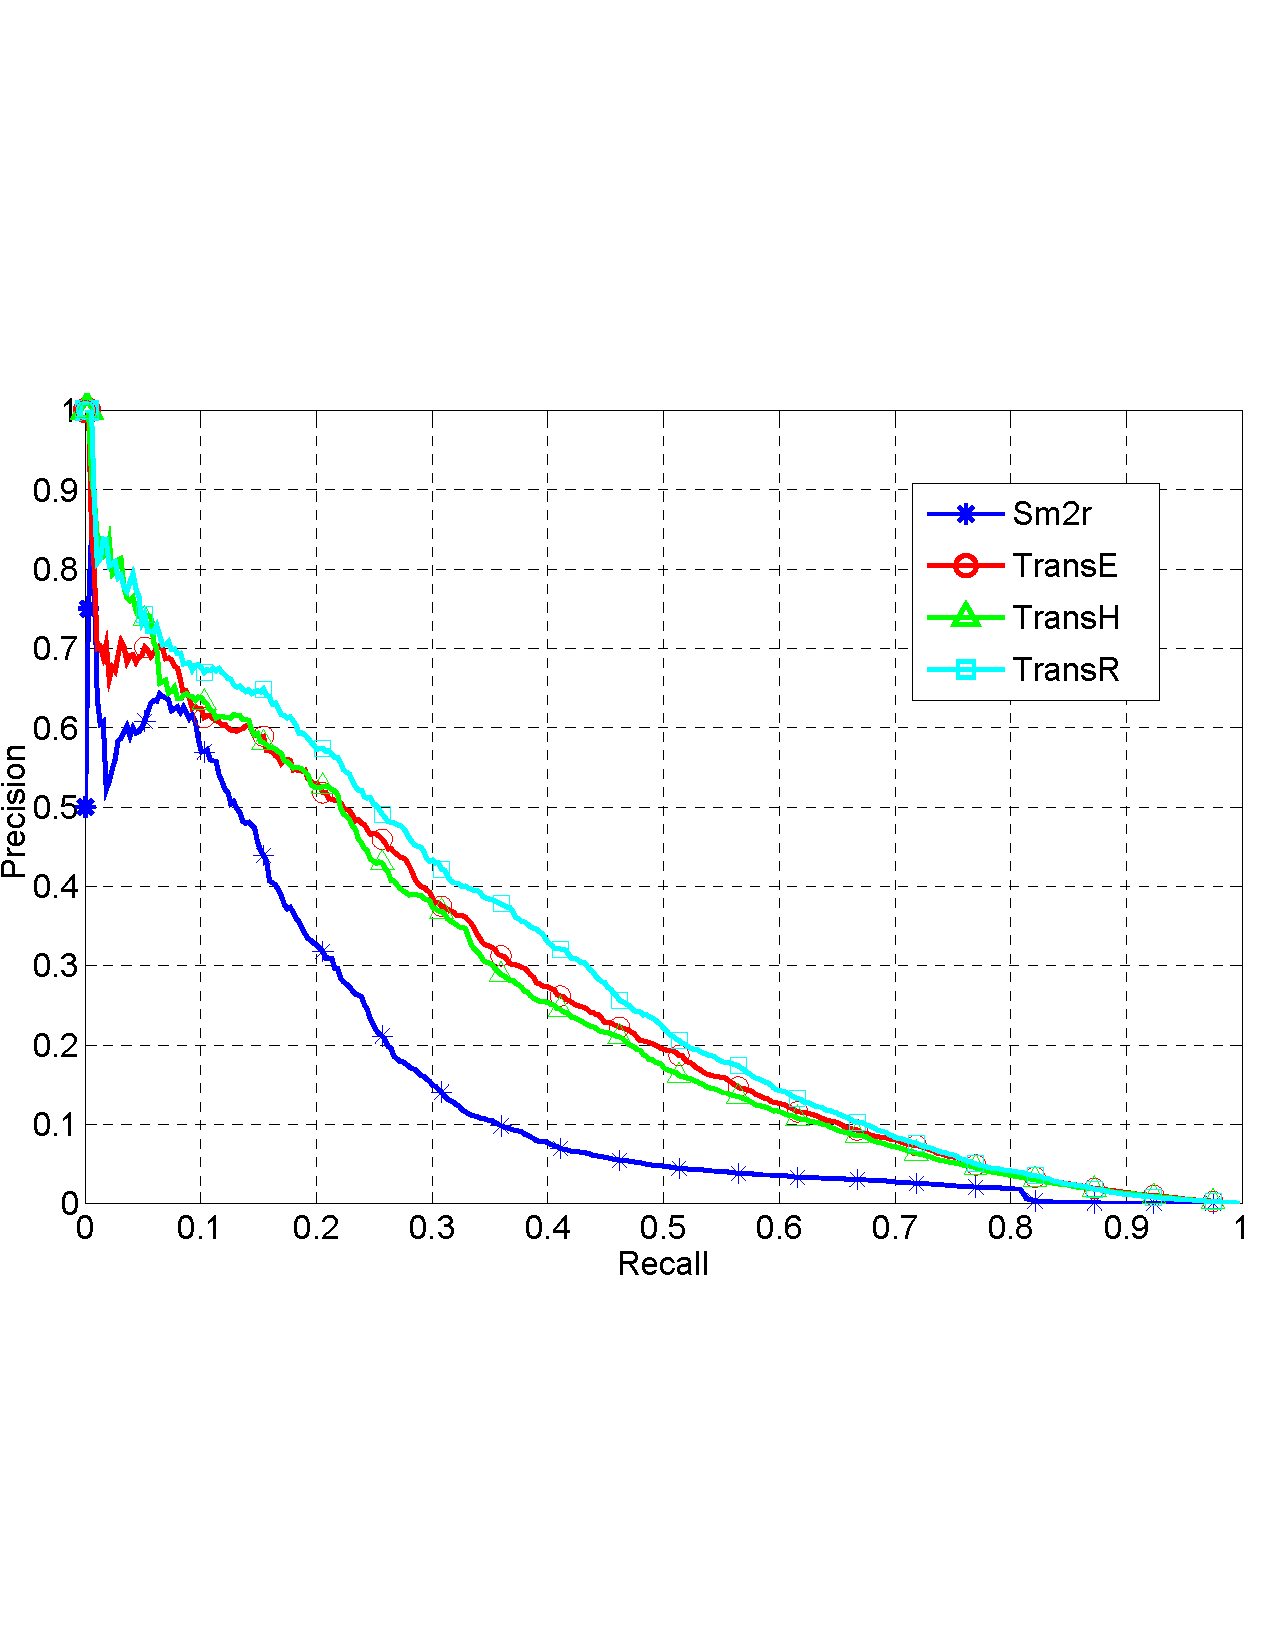
\includegraphics[width=0.8\columnwidth]{figures/trans/RE_text}
    \caption{TransE, TransH 和 TransR 在关系抽取任务上的准确召回率曲线。}
    \label{fig_1:relation_extraction}
    \end{figure}

    从表中我们观察到,当召回范围为$[0,0.05]$时,TransR 优于 TransE,与 TransH 相当,并且当召回范围为$[0.05,1]$时,则超越所有的模型,包括 TransE 和 TransH。

    最近嵌入的想法也被广泛地用于表示单词和文本的工作中 \cite{bengio2003neural,mikolov2013efficient,mikolov2013distributed,mikolov2013linguistic},这些都可以在未来用于基于文本的关系提取任务中。

    \section{结论}
    在本文中,我们提出了一种新的知识图谱嵌入模型 TransR。TransR 将实体和关系嵌入不同的实体空间和关系空间中,并通过投影实体转换到关系空间来进行学习嵌入。此外,我们还提出了 CTransR,其目的是基于分段线性回归的思想来模拟每个关系类型内部的复杂的相关性。在实验中,我们对三个任务进行评估,包括链接预测,三元组分类和文本中的关系提取。实验结果表明,与 TransE 和 TransH 相比,TransR 获得了相当一致和显著的效果改进。


% \chapter{其它附录}
% 前面两个附录主要是给本科生做例子。其它附录的内容可以放到这里,当然如果你愿意,可
% 以把这部分也放到独立的文件中,然后将其 \cs{input} 到主文件中。

\end{appendix}

%% 个人简历
% \begin{resume}

  \resumeitem{个人简历}

  1995 年 02 月 08 日出生于 江苏 省 大丰 县。

  xxxx 年 9 月考入 xx 大学 xx 系 xx 专业,xxxx 年 7 月本科毕业并获得 xx 学士学位。

  xxxx 年 9 月免试进入 xx 大学 xx 系攻读 xx 学位至今。

  \researchitem{发表的学术论文} % 发表的和录用的合在一起

  % 1. 已经刊载的学术论文(本人是第一作者,或者导师为第一作者本人是第二作者)
  \begin{publications}
    \item Yang Y, Ren T L, Zhang L T, et al. Miniature microphone with silicon-
      based ferroelectric thin films. Integrated Ferroelectrics, 2003,
      52:229-235. (SCI 收录, 检索号:758FZ.)
    \item 杨轶, 张宁欣, 任天令, 等. 硅基铁电微声学器件中薄膜残余应力的研究. 中国机
      械工程, 2005, 16(14):1289-1291. (EI 收录, 检索号:0534931 2907.)
    \item 杨轶, 张宁欣, 任天令, 等. 集成铁电器件中的关键工艺研究. 仪器仪表学报,
      2003, 24(S4):192-193. (EI 源刊.)
  \end{publications}

  % 2. 尚未刊载,但已经接到正式录用函的学术论文(本人为第一作者,或者
  %    导师为第一作者本人是第二作者)。
  \begin{publications}[before=\publicationskip,after=\publicationskip]
    \item Yang Y, Ren T L, Zhu Y P, et al. PMUTs for handwriting recognition. In
      press. (已被 Integrated Ferroelectrics 录用. SCI 源刊.)
  \end{publications}

  % 3. 其他学术论文。可列出除上述两种情况以外的其他学术论文,但必须是
  %    已经刊载或者收到正式录用函的论文。
  \begin{publications}
    \item Wu X M, Yang Y, Cai J, et al. Measurements of ferroelectric MEMS
      microphones. Integrated Ferroelectrics, 2005, 69:417-429. (SCI 收录, 检索号
      :896KM)
    \item 贾泽, 杨轶, 陈兢, 等. 用于压电和电容微麦克风的体硅腐蚀相关研究. 压电与声
      光, 2006, 28(1):117-119. (EI 收录, 检索号:06129773469)
    \item 伍晓明, 杨轶, 张宁欣, 等. 基于MEMS技术的集成铁电硅微麦克风. 中国集成电路,
      2003, 53:59-61.
  \end{publications}

  \researchitem{研究成果} % 有就写,没有就删除
  \begin{achievements}
    \item 任天令, 杨轶, 朱一平, 等. 硅基铁电微声学传感器畴极化区域控制和电极连接的
      方法: 中国, CN1602118A. (中国专利公开号)
    \item Ren T L, Yang Y, Zhu Y P, et al. Piezoelectric micro acoustic sensor
      based on ferroelectric materials: USA, No.11/215, 102. (美国发明专利申请号)
  \end{achievements}

\end{resume}


%% 本科生进行格式审查是需要下面这个表格,答辩可能不需要。选择性留下。
% 综合论文训练记录表
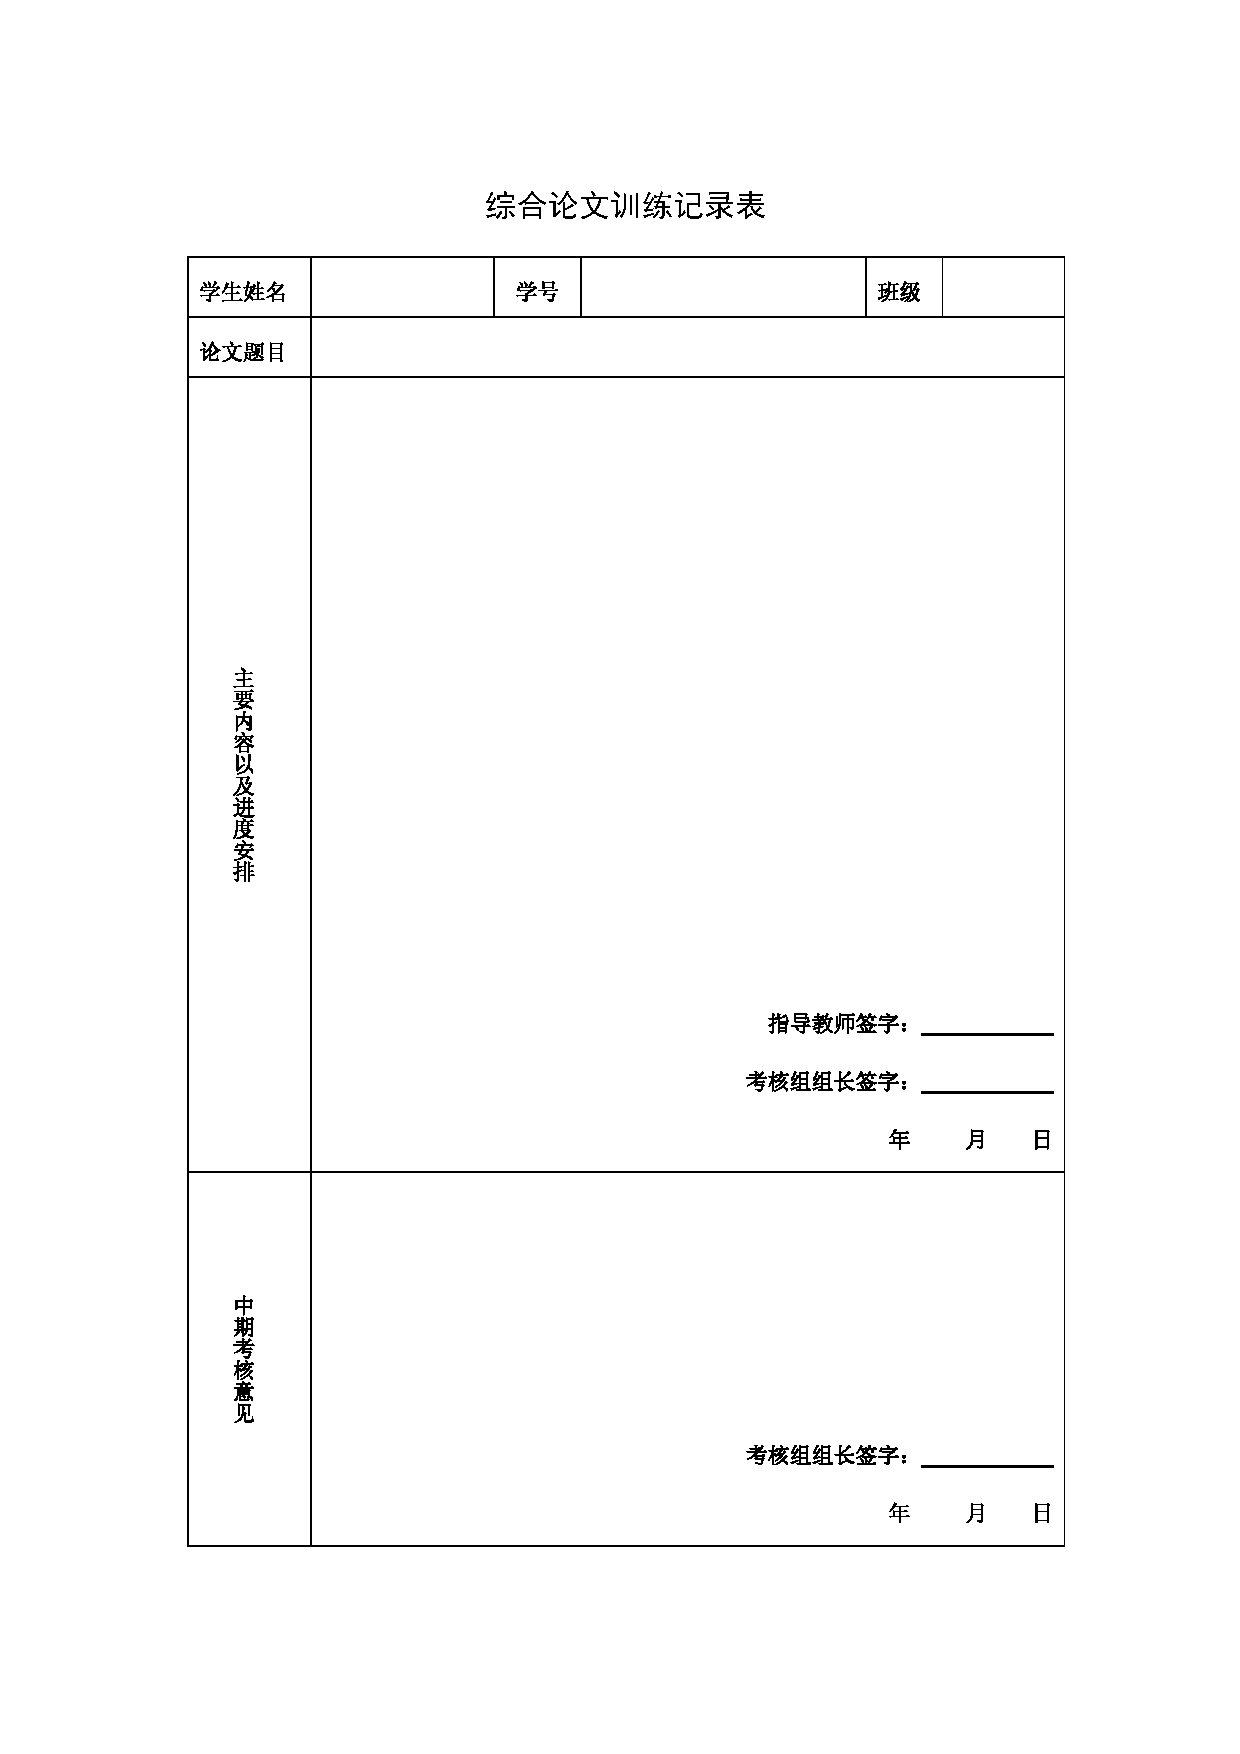
\includepdf[pages=-]{scan-record.pdf}
\end{document}
